
%% bare_jrnl_compsoc.tex
%% V1.4a
%% 2014/09/17
%% by Michael Shell
%% See:
%% http://www.michaelshell.org/
%% for current contact information.
%%
%% This is a skeleton file demonstrating the use of IEEEtran.cls
%% (requires IEEEtran.cls version 1.8a or later) with an IEEE
%% Computer Society journal paper.
%%
%% Support sites:
%% http://www.michaelshell.org/tex/ieeetran/
%% http://www.ctan.org/tex-archive/macros/latex/contrib/IEEEtran/
%% and
%% http://www.ieee.org/

%%*************************************************************************
%% Legal Notice:
%% This code is offered as-is without any warranty either expressed or
%% implied; without even the implied warranty of MERCHANTABILITY or
%% FITNESS FOR A PARTICULAR PURPOSE!
%% User assumes all risk.
%% In no event shall IEEE or any contributor to this code be liable for
%% any damages or losses, including, but not limited to, incidental,
%% consequential, or any other damages, resulting from the use or misuse
%% of any information contained here.
%%
%% All comments are the opinions of their respective authors and are not
%% necessarily endorsed by the IEEE.
%%
%% This work is distributed under the LaTeX Project Public License (LPPL)
%% ( http://www.latex-project.org/ ) version 1.3, and may be freely used,
%% distributed and modified. A copy of the LPPL, version 1.3, is included
%% in the base LaTeX documentation of all distributions of LaTeX released
%% 2003/12/01 or later.
%% Retain all contribution notices and credits.
%% ** Modified files should be clearly indicated as such, including  **
%% ** renaming them and changing author support contact information. **
%%
%% File list of work: IEEEtran.cls, IEEEtran_HOWTO.pdf, bare_adv.tex,
%%                    bare_conf.tex, bare_jrnl.tex, bare_conf_compsoc.tex,
%%                    bare_jrnl_compsoc.tex, bare_jrnl_transmag.tex
%%*************************************************************************


% *** Authors should verify (and, if needed, correct) their LaTeX system  ***
% *** with the testflow diagnostic prior to trusting their LaTeX platform ***
% *** with production work. IEEE's font choices and paper sizes can       ***
% *** trigger bugs that do not appear when using other class files.       ***                          ***
% The testflow support page is at:
% http://www.michaelshell.org/tex/testflow/


\documentclass[10pt,journal,compsoc]{IEEEtran}
%
% If IEEEtran.cls has not been installed into the LaTeX system files,
% manually specify the path to it like:
% \documentclass[10pt,journal,compsoc]{../sty/IEEEtran}





% Some very useful LaTeX packages include:
% (uncomment the ones you want to load)


% *** MISC UTILITY PACKAGES ***
%
%\usepackage{ifpdf}
% Heiko Oberdiek's ifpdf.sty is very useful if you need conditional
% compilation based on whether the output is pdf or dvi.
% usage:
% \ifpdf
%   % pdf code
% \else
%   % dvi code
% \fi
% The latest version of ifpdf.sty can be obtained from:
% http://www.ctan.org/tex-archive/macros/latex/contrib/oberdiek/
% Also, note that IEEEtran.cls V1.7 and later provides a builtin
% \ifCLASSINFOpdf conditional that works the same way.
% When switching from latex to pdflatex and vice-versa, the compiler may
% have to be run twice to clear warning/error messages.






% *** CITATION PACKAGES ***
%
\ifCLASSOPTIONcompsoc
  % IEEE Computer Society needs nocompress option
  % requires cite.sty v4.0 or later (November 2003)
  \usepackage[nocompress]{cite}
\else
  % normal IEEE
  \usepackage{cite}
\fi
% cite.sty was written by Donald Arseneau
% V1.6 and later of IEEEtran pre-defines the format of the cite.sty package
% \cite{} output to follow that of IEEE. Loading the cite package will
% result in citation numbers being automatically sorted and properly
% "compressed/ranged". e.g., [1], [9], [2], [7], [5], [6] without using
% cite.sty will become [1], [2], [5]--[7], [9] using cite.sty. cite.sty's
% \cite will automatically add leading space, if needed. Use cite.sty's
% noadjust option (cite.sty V3.8 and later) if you want to turn this off
% such as if a citation ever needs to be enclosed in parenthesis.
% cite.sty is already installed on most LaTeX systems. Be sure and use
% version 5.0 (2009-03-20) and later if using hyperref.sty.
% The latest version can be obtained at:
% http://www.ctan.org/tex-archive/macros/latex/contrib/cite/
% The documentation is contained in the cite.sty file itself.
%
% Note that some packages require special options to format as the Computer
% Society requires. In particular, Computer Society  papers do not use
% compressed citation ranges as is done in typical IEEE papers
% (e.g., [1]-[4]). Instead, they list every citation separately in order
% (e.g., [1], [2], [3], [4]). To get the latter we need to load the cite
% package with the nocompress option which is supported by cite.sty v4.0
% and later. Note also the use of a CLASSOPTION conditional provided by
% IEEEtran.cls V1.7 and later.





% *** GRAPHICS RELATED PACKAGES ***
%
\ifCLASSINFOpdf
   \usepackage[pdftex]{graphicx}
  % declare the path(s) where your graphic files are
  % \graphicspath{{../pdf/}{../jpeg/}}
  % and their extensions so you won't have to specify these with
  % every instance of \includegraphics
  % \DeclareGraphicsExtensions{.pdf,.jpeg,.png}
\else
  % or other class option (dvipsone, dvipdf, if not using dvips). graphicx
  % will default to the driver specified in the system graphics.cfg if no
  % driver is specified.
  % \usepackage[dvips]{graphicx}
  % declare the path(s) where your graphic files are
  % \graphicspath{{../eps/}}
  % and their extensions so you won't have to specify these with
  % every instance of \includegraphics
  % \DeclareGraphicsExtensions{.eps}
\fi
% graphicx was written by David Carlisle and Sebastian Rahtz. It is
% required if you want graphics, photos, etc. graphicx.sty is already
% installed on most LaTeX systems. The latest version and documentation
% can be obtained at:
% http://www.ctan.org/tex-archive/macros/latex/required/graphics/
% Another good source of documentation is "Using Imported Graphics in
% LaTeX2e" by Keith Reckdahl which can be found at:
% http://www.ctan.org/tex-archive/info/epslatex/
%
% latex, and pdflatex in dvi mode, support graphics in encapsulated
% postscript (.eps) format. pdflatex in pdf mode supports graphics
% in .pdf, .jpeg, .png and .mps (metapost) formats. Users should ensure
% that all non-photo figures use a vector format (.eps, .pdf, .mps) and
% not a bitmapped formats (.jpeg, .png). IEEE frowns on bitmapped formats
% which can result in "jaggedy"/blurry rendering of lines and letters as
% well as large increases in file sizes.
%
% You can find documentation about the pdfTeX application at:
% http://www.tug.org/applications/pdftex






% *** MATH PACKAGES ***
%
\usepackage[cmex10]{amsmath}
% A popular package from the American Mathematical Society that provides
% many useful and powerful commands for dealing with mathematics. If using
% it, be sure to load this package with the cmex10 option to ensure that
% only type 1 fonts will utilized at all point sizes. Without this option,
% it is possible that some math symbols, particularly those within
% footnotes, will be rendered in bitmap form which will result in a
% document that can not be IEEE Xplore compliant!
%
% Also, note that the amsmath package sets \interdisplaylinepenalty to 10000
% thus preventing page breaks from occurring within multiline equations. Use:
\interdisplaylinepenalty=2500
% after loading amsmath to restore such page breaks as IEEEtran.cls normally
% does. amsmath.sty is already installed on most LaTeX systems. The latest
% version and documentation can be obtained at:
% http://www.ctan.org/tex-archive/macros/latex/required/amslatex/math/
\usepackage{color}
\usepackage{overpic}
\usepackage[normalem]{ulem}
\usepackage{soul}
\usepackage{amsfonts}
\usepackage{wrapfig}
\usepackage{algorithm}
\usepackage{algorithmic}
%\usepackage{algorithmicx}
%\usepackage{algpseudocode}
\usepackage{amssymb}
\usepackage{enumitem}

\usepackage{graphicx}
\usepackage{subfigure}
\usepackage{multirow}



\usepackage{balance}  % to better equalize the last page
\usepackage{times}    % comment if you want LaTeX's default font
\renewcommand{\algorithmicrequire}{\textbf{Input:}}  %Use Input in the format of Algorithm
\renewcommand{\algorithmicensure}{\textbf{Output:}} %UseOutput in the format of Algorithm

\newcommand\tabhead[1]{\small\textbf{#1}}

\usepackage{customized_commands}



% *** SPECIALIZED LIST PACKAGES ***
%
%\usepackage{algorithmic}
% algorithmic.sty was written by Peter Williams and Rogerio Brito.
% This package provides an algorithmic environment fo describing algorithms.
% You can use the algorithmic environment in-text or within a figure
% environment to provide for a floating algorithm. Do NOT use the algorithm
% floating environment provided by algorithm.sty (by the same authors) or
% algorithm2e.sty (by Christophe Fiorio) as IEEE does not use dedicated
% algorithm float types and packages that provide these will not provide
% correct IEEE style captions. The latest version and documentation of
% algorithmic.sty can be obtained at:
% http://www.ctan.org/tex-archive/macros/latex/contrib/algorithms/
% There is also a support site at:
% http://algorithms.berlios.de/index.html
% Also of interest may be the (relatively newer and more customizable)
% algorithmicx.sty package by Szasz Janos:
% http://www.ctan.org/tex-archive/macros/latex/contrib/algorithmicx/




% *** ALIGNMENT PACKAGES ***
%
%\usepackage{array}
% Frank Mittelbach's and David Carlisle's array.sty patches and improves
% the standard LaTeX2e array and tabular environments to provide better
% appearance and additional user controls. As the default LaTeX2e table
% generation code is lacking to the point of almost being broken with
% respect to the quality of the end results, all users are strongly
% advised to use an enhanced (at the very least that provided by array.sty)
% set of table tools. array.sty is already installed on most systems. The
% latest version and documentation can be obtained at:
% http://www.ctan.org/tex-archive/macros/latex/required/tools/


% IEEEtran contains the IEEEeqnarray family of commands that can be used to
% generate multiline equations as well as matrices, tables, etc., of high
% quality.




% *** SUBFIGURE PACKAGES ***
%\ifCLASSOPTIONcompsoc
%  \usepackage[caption=false,font=footnotesize,labelfont=sf,textfont=sf]{subfig}
%\else
%  \usepackage[caption=false,font=footnotesize]{subfig}
%\fi
% subfig.sty, written by Steven Douglas Cochran, is the modern replacement
% for subfigure.sty, the latter of which is no longer maintained and is
% incompatible with some LaTeX packages including fixltx2e. However,
% subfig.sty requires and automatically loads Axel Sommerfeldt's caption.sty
% which will override IEEEtran.cls' handling of captions and this will result
% in non-IEEE style figure/table captions. To prevent this problem, be sure
% and invoke subfig.sty's "caption=false" package option (available since
% subfig.sty version 1.3, 2005/06/28) as this is will preserve IEEEtran.cls
% handling of captions.
% Note that the Computer Society format requires a sans serif font rather
% than the serif font used in traditional IEEE formatting and thus the need
% to invoke different subfig.sty package options depending on whether
% compsoc mode has been enabled.
%
% The latest version and documentation of subfig.sty can be obtained at:
% http://www.ctan.org/tex-archive/macros/latex/contrib/subfig/





% *** FLOAT PACKAGES ***
%
%\usepackage{fixltx2e}
% fixltx2e, the successor to the earlier fix2col.sty, was written by
% Frank Mittelbach and David Carlisle. This package corrects a few problems
% in the LaTeX2e kernel, the most notable of which is that in current
% LaTeX2e releases, the ordering of single and double column floats is not
% guaranteed to be preserved. Thus, an unpatched LaTeX2e can allow a
% single column figure to be placed prior to an earlier double column
% figure. The latest version and documentation can be found at:
% http://www.ctan.org/tex-archive/macros/latex/base/


%\usepackage{stfloats}
% stfloats.sty was written by Sigitas Tolusis. This package gives LaTeX2e
% the ability to do double column floats at the bottom of the page as well
% as the top. (e.g., "\begin{figure*}[!b]" is not normally possible in
% LaTeX2e). It also provides a command:
%\fnbelowfloat
% to enable the placement of footnotes below bottom floats (the standard
% LaTeX2e kernel puts them above bottom floats). This is an invasive package
% which rewrites many portions of the LaTeX2e float routines. It may not work
% with other packages that modify the LaTeX2e float routines. The latest
% version and documentation can be obtained at:
% http://www.ctan.org/tex-archive/macros/latex/contrib/sttools/
% Do not use the stfloats baselinefloat ability as IEEE does not allow
% \baselineskip to stretch. Authors submitting work to the IEEE should note
% that IEEE rarely uses double column equations and that authors should try
% to avoid such use. Do not be tempted to use the cuted.sty or midfloat.sty
% packages (also by Sigitas Tolusis) as IEEE does not format its papers in
% such ways.
% Do not attempt to use stfloats with fixltx2e as they are incompatible.
% Instead, use Morten Hogholm'a dblfloatfix which combines the features
% of both fixltx2e and stfloats:
%
% \usepackage{dblfloatfix}
% The latest version can be found at:
% http://www.ctan.org/tex-archive/macros/latex/contrib/dblfloatfix/




%\ifCLASSOPTIONcaptionsoff
%  \usepackage[nomarkers]{endfloat}
% \let\MYoriglatexcaption\caption
% \renewcommand{\caption}[2][\relax]{\MYoriglatexcaption[#2]{#2}}
%\fi
% endfloat.sty was written by James Darrell McCauley, Jeff Goldberg and
% Axel Sommerfeldt. This package may be useful when used in conjunction with
% IEEEtran.cls'  captionsoff option. Some IEEE journals/societies require that
% submissions have lists of figures/tables at the end of the paper and that
% figures/tables without any captions are placed on a page by themselves at
% the end of the document. If needed, the draftcls IEEEtran class option or
% \CLASSINPUTbaselinestretch interface can be used to increase the line
% spacing as well. Be sure and use the nomarkers option of endfloat to
% prevent endfloat from "marking" where the figures would have been placed
% in the text. The two hack lines of code above are a slight modification of
% that suggested by in the endfloat docs (section 8.4.1) to ensure that
% the full captions always appear in the list of figures/tables - even if
% the user used the short optional argument of \caption[]{}.
% IEEE papers do not typically make use of \caption[]'s optional argument,
% so this should not be an issue. A similar trick can be used to disable
% captions of packages such as subfig.sty that lack options to turn off
% the subcaptions:
% For subfig.sty:
% \let\MYorigsubfloat\subfloat
% \renewcommand{\subfloat}[2][\relax]{\MYorigsubfloat[]{#2}}
% However, the above trick will not work if both optional arguments of
% the \subfloat command are used. Furthermore, there needs to be a
% description of each subfigure *somewhere* and endfloat does not add
% subfigure captions to its list of figures. Thus, the best approach is to
% avoid the use of subfigure captions (many IEEE journals avoid them anyway)
% and instead reference/explain all the subfigures within the main caption.
% The latest version of endfloat.sty and its documentation can obtained at:
% http://www.ctan.org/tex-archive/macros/latex/contrib/endfloat/
%
% The IEEEtran \ifCLASSOPTIONcaptionsoff conditional can also be used
% later in the document, say, to conditionally put the References on a
% page by themselves.




% *** PDF, URL AND HYPERLINK PACKAGES ***
%
%\usepackage{url}
% url.sty was written by Donald Arseneau. It provides better support for
% handling and breaking URLs. url.sty is already installed on most LaTeX
% systems. The latest version and documentation can be obtained at:
% http://www.ctan.org/tex-archive/macros/latex/contrib/url/
% Basically, \url{my_url_here}.





% *** Do not adjust lengths that control margins, column widths, etc. ***
% *** Do not use packages that alter fonts (such as pslatex).         ***
% There should be no need to do such things with IEEEtran.cls V1.6 and later.
% (Unless specifically asked to do so by the journal or conference you plan
% to submit to, of course. )


% correct bad hyphenation here
\hyphenation{op-tical net-works semi-conduc-tor}

\newcommand{\shortcite}[1]{\cite{#1}}
\newcommand{\figref}[1]{Figure~\ref{#1}}
\newcommand{\tabref}[1]{Table~\ref{#1}}
\newcommand{\eqnref}[1]{Eq.~\eqref{#1}}
\newcommand{\secref}[1]{Section~\ref{#1}}
\newcommand{\appref}[1]{Appendix~\ref{#1}}
\newcommand{\lstref}[1]{Algorithm~\ref{#1}}
\newcommand{\tab}[1]{\mathbf{#1}}
\newcommand{\comments}[1]{}
\newcommand{\ZK}[1]{\textcolor[rgb]{1.00,0.00,0.0}{#1}}

\newcommand{\mypara}[1]{\vspace{0.05in}\noindent\textbf{#1.}}
\newcommand{\comment}[1]{\textcolor[rgb]{0,0,1}{\textbf{#1}}}
\newcommand{\niloy}[1]{{\color{red}\bf{NM: #1}}}

%\newcommand{\youyi}[1]{{\color{magenta}\bf{youyi: #1}}}
\newcommand{\mcc}[1]{{\color{cyan}\bf{#1}}}


\newcommand{\vnudge}{\vspace{-.1in}}
%\newcommand{\vv}[1]{\ensuremath{\mathbf{#1}}}

%% this command may change the "noindent" properties.
\newcommand{\ldpswap}[2]{{\sout{#1}}{\textcolor[rgb]{0,0.65,0.32}{#2}}}
\newcommand{\stjswap}[2]{{\sout{#1}}{\textcolor[rgb]{0,0,1}{#2}}}
\newcommand{\hongzhicomment}[1]{\textcolor[rgb]{0.65,0.32, 0}{#1}}
%\DeclareMathOperator*{\argmin}{\arg\!\min}
%\DeclareMathOperator*{\argmax}{\arg\!\max}

\begin{document}
%
% paper title
% Titles are generally capitalized except for words such as a, an, and, as,
% at, but, by, for, in, nor, of, on, or, the, to and up, which are usually
% not capitalized unless they are the first or last word of the title.
% Linebreaks \\ can be used within to get better formatting as desired.
% Do not put math or special symbols in the title.
\title{Toward Support-free 3{D} Printing:\\ A skeletal Approach for Partitioning Models}
%
%
% author names and IEEE memberships
% note positions of commas and nonbreaking spaces ( ~ ) LaTeX will not break
% a structure at a ~ so this keeps an author's name from being broken across
% two lines.
% use \thanks{} to gain access to the first footnote area
% a separate \thanks must be used for each paragraph as LaTeX2e's \thanks
% was not built to handle multiple paragraphs
%
%
%\IEEEcompsocitemizethanks is a special \thanks that produces the bulleted
% lists the Computer Society journals use for "first footnote" author
% affiliations. Use \IEEEcompsocthanksitem which works much like \item
% for each affiliation group. When not in compsoc mode,
% \IEEEcompsocitemizethanks becomes like \thanks and
% \IEEEcompsocthanksitem becomes a line break with idention. This
% facilitates dual compilation, although admittedly the differences in the
% desired content of \author between the different types of papers makes a
% one-size-fits-all approach a daunting prospect. For instance, compsoc
% journal papers have the author affiliations above the "Manuscript
% received ..."  text while in non-compsoc journals this is reversed. Sigh.

\author{Xiangzhi~Wei \quad
        Siqi~Qiu \quad
        Lin Zhu\quad
        Juntong Xi\quad
        Youyi~Zheng\thanks{$\dag$ corresponding author}$^{\dag}$
\IEEEcompsocitemizethanks{\IEEEcompsocthanksitem X. Wei, S. Qiu, L. Zhu and J. Xi are with the Department of Intelligent Manufacturing and Information Engineering, School of Mechanical Engineering,Shanghai Jiao Tong University, China.\protect\\
% note need leading \protect in front of \\ to get a newline within \thanks as
% \\ is fragile and will error, could use \hfil\break instead.
E-mail: ~\{antonwei,siqiqiu,zhulin0728,jtxi\}@sjtu.edu.cn
\IEEEcompsocthanksitem Youyi~Zheng is with ShanghaiTech University, China.\protect\\
E-mail: ~zhengyy@shanghaitech.edu.cn
}% <-this % stops an unwanted space
%\thanks{Manuscript received April 19, 2005; revised September 17, 2014.}
}


% note the % following the last \IEEEmembership and also \thanks -
% these prevent an unwanted space from occurring between the last author name
% and the end of the author line. i.e., if you had this:
%
% \author{....lastname \thanks{...} \thanks{...} }
%                     ^------------^------------^----Do not want these spaces!
%
% a space would be appended to the last name and could cause every name on that
% line to be shifted left slightly. This is one of those "LaTeX things". For
% instance, "\textbf{A} \textbf{B}" will typeset as "A B" not "AB". To get
% "AB" then you have to do: "\textbf{A}\textbf{B}"
% \thanks is no different in this regard, so shield the last } of each \thanks
% that ends a line with a % and do not let a space in before the next \thanks.
% Spaces after \IEEEmembership other than the last one are OK (and needed) as
% you are supposed to have spaces between the names. For what it is worth,
% this is a minor point as most people would not even notice if the said evil
% space somehow managed to creep in.



% The paper headers
\markboth{\emph{IEEE} TRANSACTIONS ON VISUALIZATION AND COMPUTER GRAPHICS, VOL. XX, NO. XX }%
{Shell \MakeLowercase{\textit{et al.}}: Bare Demo of IEEEtran.cls for Computer Society Journals}
% The only time the second header will appear is for the odd numbered pages
% after the title page when using the twoside option.
%
% *** Note that you probably will NOT want to include the author's ***
% *** name in the headers of peer review papers.                   ***
% You can use \ifCLASSOPTIONpeerreview for conditional compilation here if
% you desire.



% The publisher's ID mark at the bottom of the page is less important with
% Computer Society journal papers as those publications place the marks
% outside of the main text columns and, therefore, unlike regular IEEE
% journals, the available text space is not reduced by their presence.
% If you want to put a publisher's ID mark on the page you can do it like
% this:
%\IEEEpubid{0000--0000/00\$00.00~\copyright~2014 IEEE}
% or like this to get the Computer Society new two part style.
%\IEEEpubid{\makebox[\columnwidth]{\hfill 0000--0000/00/\$00.00~\copyright~2014 IEEE}%
%\hspace{\columnsep}\makebox[\columnwidth]{Published by the IEEE Computer Society\hfill}}
% Remember, if you use this you must call \IEEEpubidadjcol in the second
% column for its text to clear the IEEEpubid mark (Computer Society jorunal
% papers don't need this extra clearance.)



% use for special paper notices
%\IEEEspecialpapernotice{(Invited Paper)}



% for Computer Society papers, we must declare the abstract and index terms
% PRIOR to the title within the \IEEEtitleabstractindextext IEEEtran
% command as these need to go into the title area created by \maketitle.
% As a general rule, do not put math, special symbols or citations
% in the abstract or keywords.
\IEEEtitleabstractindextext{%
\begin{abstract}
We propose an algorithm for partitioning a 3{D} model into the least number of parts for 3{D} printing without using any support structure. Minimizing support structures is crucial in reducing 3D printing material and time, partition-based methods are efficient means in realizing this objective. Although there exists some algorithm for support-free fabrication of solid models, no algorithm ever considers the problem of support-free fabrication for 3D printed shell models. Any partition will inevitably induce seams and cracks on the assembled model, which affects the aesthetics and strength of the finished surface. In this paper, to achieve support-free fabrication while minimizing the effect of the seams, we put forward an optimization system with the minimization of the number of partitioned components and the total length of the cuts, under the constraints of support-free printing angle. Our approach is particularly efficient for shell models, and it can be applicable to solid models as well. We show that the optimization problem is {NP}-hard and propose a Monte Carlo method to find an {optimal} solution to the objectives. We applied our partition method on a number of 3{D} models. Finally, we validate our method by carrying out a serial of 3D printing experiments.
\end{abstract}

% Note that keywords are not normally used for peerreview papers.
\begin{IEEEkeywords}
3D printing, skeleton, model partition, support-free.
\end{IEEEkeywords}}


% make the title area
\maketitle


% To allow for easy dual compilation without having to reenter the
% abstract/keywords data, the \IEEEtitleabstractindextext text will
% not be used in maketitle, but will appear (i.e., to be "transported")
% here as \IEEEdisplaynontitleabstractindextext when the compsoc
% or transmag modes are not selected <OR> if conference mode is selected
% - because all conference papers position the abstract like regular
% papers do.
\IEEEdisplaynontitleabstractindextext
% \IEEEdisplaynontitleabstractindextext has no effect when using
% compsoc or transmag under a non-conference mode.



% For peer review papers, you can put extra information on the cover
% page as needed:
% \ifCLASSOPTIONpeerreview
% \begin{center} \bfseries EDICS Category: 3-BBND \end{center}
% \fi
%
% For peerreview papers, this IEEEtran command inserts a page break and
% creates the second title. It will be ignored for other modes.
\IEEEpeerreviewmaketitle


% Computer Society journal (but not conference!) papers do something unusual
% with the very first section heading (almost always called "Introduction").
% They place it ABOVE the main text! IEEEtran.cls does not automatically do
% this for you, but you can achieve this effect with the provided
% \IEEEraisesectionheading{} command. Note the need to keep any \label that
% is to refer to the section immediately after \section in the above as
% \IEEEraisesectionheading puts \section within a raised box.
\section{Introduction}

3D printing, or additive manufacturing, has drawn growing interests from researchers in computer graphics. Fused deposition modeling (FDM), stereolithographic (SLA), Selective Laser Melting (SLM) and Selective Laser Sintering (SLS) and the four most popular means of 3D printing techniques. Although 3D printing has seen its applications in producing arbitrarily intricate 3D models, the price of the printing materials, especially for those with high quality, are still outrageously high. Therefore, it is desirable to reduce materials used in the fabrication process. Note that this is also a critical operation for reducing production time and therefore the total production cost. For this purpose, an efficient method is to minimize the support structures, which are removed in the post-processing phase of the fabrication task.

As for minimizing support structures, Autodesk R MeshMixerTM provides a semiautomatic orientation optimization tool to minimize support volume, support area, structural strength, or a combination of these three attributes. However, it requires professional experience in setting the geometric parameters manually. A number of literatures have studied various factors that influence the volume of supports, e.g., optimizing the topology of the support structure \cite{DumasHL14,VanekGB14}, determining an optimal fabrication direction \cite{Zhang:2015,HildebrandBA13,padhye2011multi}, partitioning any given model into a set of separate parts that satisfy particular geometric properties such as being pyramidical \cite{Hu_siga14}, has minimal packing volume \cite{VanekGBMCSM14} or inter-lockable \cite{SongFLF15}. However, the partition results of these methods do not simultaneously respect the geometric properties and the support-free printability of the portioned parts. Further, no existing methods ever consider the problem of partitioning a boundary-represented mesh into the least number of parts whose fabrication is free of support structures. The least number of portioned parts corresponds to the least number of seams on the final assembled model, which ensures a nice aesthetics preservation of the model surface; and the support-free fabrication saves material to the most extent, which is particularly helpful in printing objects made of metal powder, resin, or nice plastics, etc.

This paper addresses the problem of decomposing a 3{D} model into the least number of parts, each of which, when printed in a proper direction, is free of support materials. Unfortunately, this problem is identical to the multi-container packing problem, which has been shown to be NP-hard \cite{Fukunaga:2007}. Our solution of the problem draws inspiration from the 1{D} representation of organic models, i.e., skeletons: the topology variations of a natural model can be well-encoded by its skeleton, and a segment of the skeleton corresponding to a chunk of a mesh; further, the mesh chunk is typically a cylinder-like shape which can be printed free of support structures if the printing direction is parallel to the skeletal direction.

We restrict our focus on organic or man-made models since those shapes merit well-defined skeletons. Further, support structures are required for the interior and exterior surface of a mesh model during the 3{D} printing process. Our approach assumes that the interior of a mesh model is hollowed and the mesh model is shelled with a printer-friendly thickness. Therefore, our objective is to partition a model according to the growth of its skeleton into a set of sub-parts, such that each sub-part is represented by a skeletal subgraph which can be fabricated in a good printing direction without any support structure. In the meanwhile, we also look for a best set of partitioned sub-parts which induce the minimal partition length.

Formally, given a printing direction, if the angle between a facet and the printing direction is less than or equal to $\theta$ which is a printer-dependent value, then the facet can be printed without using any support structure. This inspires us to compute a minimum set of subgraph of the skeleton, such that each edge in any subgraph subtends to an axis (the printing direction) by an angle of no larger than $\theta$, the corresponding chunk of the mesh is therefore support-free as printed along this axis. In general, a cone of axes satisfies this angle constraint.

%However, the volume of the chunk should be within the working space of the printer. Further, if the center of mass of the chunk diverts from the support center too much, e.g., the gravitational torque applied at the mass center is too far away from the center of support that it bends the printing model by a layer of thickness, then the surface quality of the model is poor or the printing task fails since the next printing layer cannot be firmly attached to the previous layer.

Our method handles this issue in a unified Monte Carlo framework which simultaneously looks for the best set of subgraphs which is support-free and with minimal partition length.

In short, our method makes the following contributions:

\begin{itemize}
\item {We partition any given mesh model into the least number of parts that are printable free of support structures; meanwhile, we preserve the aesthetics of the surface with the least number of seams whose length is minimized.}
\item {We propose a Monte Carlo graph partition method based on the guide of 1D Laplacian skeleton of a given mesh model.}
\end{itemize}


\section{Related Work}

Our work is focused on model partition, with the particular purpose for support-free fabrication. Here we briefly review a set of most relevant recent works.

\textbf{Computational Fabrication.} Recently, an increasing body of research work has been devoted to computational fabrication using 3{D} printing as the emergence of advanced 3{D} printing devices. In computer graphics, a number of literatures have focused on the fabrication of 3{D} models using 3{D} printers. Optimization works have been devoted to structural designs with emphasis on saving printing materials while preserving certain strength \cite{StavaVBCM12,ZhouPZ13,WangWYLTTDCL13,Umetani:2013:CSA,wang2013cost,LuSZWFCSTCC14,hornus2015tight,xie2017support}. The printability of critical structures (e.g., bridges, spikes, holes, etc.) during the FDM processes has been investigated \cite{telea2011voxel,DumasHL14}. The modeling of some particular features have also been studied, for example, surface quality \cite{wang2016improved}, deformation behavior \cite{SkourasTCBG13}, animated mechanical characters \cite{CorosTNSFSMB13,CeylanLMAP13}, articulated models with mobile joints \cite{BacherBJP12,CaliCAKSKW12}, models spinnable motions \cite{Bacher14}, and self-balancing \cite{PrevostWLS13}.

\textbf{Shape Decomposition.} In geometry processing, decomposing a shape into meaningful parts is a fundamental problem \cite{Kaick:2014:SSA}. Many efforts have been devoted to the problem of model decomposition. An excellent survey can be found in \cite{Shamir08}. A large body of research are focusing on partitioning a given 3{D} model into parts which agree with human perception \cite{KatzT03,KatzLT05,JiLCW06,LiuZ07,Golovinskiy:2008,ChenGF09,KaickFKAC14}, among which geometric features captures shape concaveness are mostly exploited in accordance with the minima rules \cite{hoffman1984parts,hoffman1997salience}. Other approaches are more application-oriented. For example, texture mapping techniques often require the input shape being decomposed into charts which can be flatten to match image textures \cite{zhou2004iso,Garcia:2008:IIG}. Our method of partition is based on shape skeletons. Although there has been previous work on skeleton based shape decomposition \cite{lien2006simultaneous,reniers2007skeleton,AuTCCL08}, none of them is designed for support-free fabrication.


\textbf{Fabrication-driven Model Partition.} A 3{D} printer cannot directly print a model whose size is larger than the printer's working space. To overcome this practical limitation, Luo et al. \cite{LuoBRM12} proposed a solution to partition a given 3D model into parts for 3D printing and then assemble the parts together. This approach has a few advantages: (i) it is cost-effective in the sense that we only need to print a replacement part for a corresponding broken part; (ii) it is convenient for storage and transportation; (iii) changing some parts of a model allows innovative designs. Along this line of research, Hao et al. \cite{hao2011efficient} partitioned a large complex model into simpler 3D printable parts by using curvature-based partitioning. Hildebrand et al. \cite{HildebrandBA13} addressed the directional bias issue in 3D printing by segmenting a 3D model into a few parts each of which is assigned an optimal printing orientation. Vanek et al. \cite{VanekGBMCSM14} reduced the time and material cost of 3D printing by hollowing a 3D model into shells and breaking them into parts, a number of parameters including the total connecting area and volume of each segment are considered during the optimization process. Attene et al. \cite{attene2015shapes} introduced a method for decomposing a model into parts which can be packed in a box. Yao et al. \cite{yao2015level} further investigated the problem of optimized partition and packing by considering multiple metrics and integrated level-set methods into a unified framework. Song et al. \cite{SongFLF15} recently developed a novel voxelization-based approach to construct inter-locking 3D parts from a given 3D model. In their later work, Song et al. \cite{song2016cofifab} combined 3D printing and 2D laser cutting for cost-effective fabrication of large objects. Without using any glue, Xin et al. \cite{XinLFWHC11} and Song et al. \cite{SongFC12} took a 3D interlocking approach to construct and connect printed 3D parts to form an object assembly. None of these methods considers the problem of support-free fabrication. Most recently, Hu et al. \cite{Hu_siga14} proposed an nice algorithm for decomposing a solid model into the least number of pyramids, each of which can be fabricated without support material. However, their algorithm is only designed for volumetric models while our algorithm aims for both shell and solid models.









\section{Overview}

In nature, most organic models ubiquitously contain cylindrical parts \cite{Zhou:2015:GCD}, e.g., arms, legs, etc. Moreover, an cylindrical part can be well represented by its corresponding 1{D} skeleton. Based on this property, a chunk of a mesh model can be fabricated free of support {if all the arcs of its corresponding skeleton piece subtend to a printing direction by an angle of no large than $\theta$.} Hence, our problem becomes partitioning a given 1{D} skeleton graph into a set of subgraphs such that each subgraph merits the desirable support-free property. In the remainder of the paper, by model we mean an organic mesh model of natural life form or articulated figures preserving nice topology features of real lives.

\textbf{Choise of skeleton.} Compared to natural skeletons, the medial axis can describe the topology of a mesh model more precisely \cite{ZhangXWYTW15}. However, a medial axis of a 3D mesh model is a 2D surface which cannot be conveniently applied to describe the critical topology changes of the model. Additionally, the medial axis consists of intersecting pieces of planes and conic surfaces, presenting significant complications to algorithms that attempt to construct 3D medial axes.
Reeb graph provides a possible choice for 1D skeleton. During the generation process of any reeb graph, the slicing direction and the position of the representative node on each slide (a connected region) seriously influence the choice of critical points and therefore generation of the Reeb graph. However, the determination of suitable slicing direction and representative nodes is an intractable problem. We resort to the 1D Laplacian skeleton proposed by \cite{AuTCCL08} which is extracted by shrinking the mesh model using Laplacian smoothing, such 1D Laplacian skeleton provides an excellent choice for reasonably describing the geometrical and topological variations of any 3{D} model.

%Figure \ref{fig:ex1} shows an example of the Laplacian skeleton.

%\begin{figure}[tbp]
%  \centering
% \mbox{} \hfill
%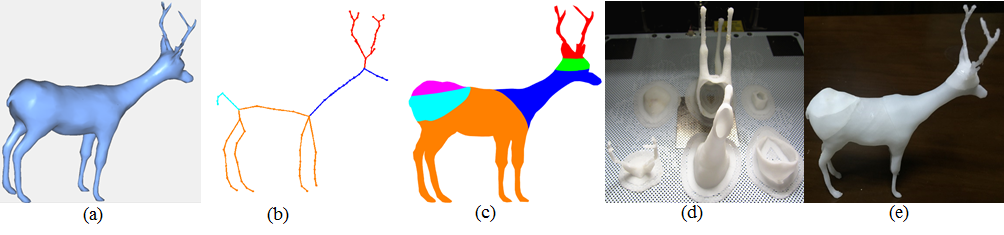
\includegraphics[width=0.4\textwidth]{figs/tree_with_skeleton.png}
%\caption{\label{fig:ex1}%
%        An illustration of a 3D mesh model and its 1D Laplacian skeleton. }
%\end{figure}



\textbf{Problem Statement.} Our goal is hence to decompose the 1D Laplacian skeleton of the model into {{a proper number of support-free subgraphs leads to a partition of the model into the least printable parts free of support structures and seams on the final assembled model.}} In addition, since support structures result in bumpy supported areas, support-free fabrication also means a nice preservation of the surface quality of the parts. Further, a minimization of the number of cuts and the total cutting length means a minimum amount of seams and their lengths on the assembled model. Therefore, we focus on these two problems in this paper.

{\color{blue}{Finding a decomposition of the skeleton into the least pieces of support free subgraphs is a non-trivial task. As a simple example, {{suppose for simplicity that the least number of cuts on the skeleton corresponds to the least number of cuts on the mesh model}}, refer to Figure \ref{fig:fork}, consider a 1{D} Laplacian skeleton that is a fork with $n$ arcs sharing a common origin; consider partitioning the fork into the least number of sub-forks such that each sub-fork can be packed into a cone of angle $2\theta$ in order to make the sub-fork support-free when fabricated in a given direction, where $\theta$ is defined based on the printing experiments as a safe angle allowing support-free fabrication.

\emph{\textbf{Theorem 1}: Partitioning a graph into the least number of support-free subgraphs is NP-hard.}

\emph{Proof}:
We shall complete the proof by transforming an instance of a known $NP$ hard problem into our problem in polynomial time.
First we need to show that our problem is in $NP$: The certificate is a set of arc-disjoint and rooted subgraphs of the input graph (skeleton), a certifier checks in polynomial time (i.e., $O(n^2)$) that the number of subgraphs is at most the given bound $K$, and that the rooted subgraphs satisfy the angle constraint of $2\theta$.
We shall reduce the Clique Cover problem to the skeleton partition problem, where the Clique Cover problem is covering a graph with the least number of cliques (complete graphs), which has been shown to be $NP$-hard [Karp]. We now show that Clique Cover ��$p$ Skeleton Partition. We define the following instance of Clique Cover: an arbitrary planar $G(V, E)$ such that $|V| = n$ and each pair of nodes ($v_i$, $v_j$) is connected by an arc if $|v_iv_j|$ is no larger than a given bound $D$. Then construct a skeleton $S$ of $n$ arcs rooted at a common node as follows: select any triplet of nodes {$v_i$, $v_j$, $v_k$} from $G$ and construct a triplet of unit arcs $\{e_i, e_j, e_k\}$ in $S$, the angle between each pair of arcs $\{e_i, e_j\}$, denoted as $A(e_i, e_j)$, is defined as $A(e_i, e_j) = 2\theta|v_iv_j|/D$. See Figure \ref{fig:fork}, given this triplet of arcs as the basis (three distinct vectors in 3{D} space), we can construct each of the remaining arcs of $S$, denoted as $e_x$, which represents a node $v_x$ in $G$: the relative position of $e_x$ with respect to each element of $\{e_i, e_j, e_k\}$ is defined as the distance from $v_x$ to each element of $\{v_i, v_j, v_k\}$. This transformation takes $O(n^2)$ time.

%Youyi: please add in the following ref. [Karp] Karp, Richard, "Reducibility Among Combinatorial Problems", in Miller, R. E.; Thatcher, J. W., Proceedings of a Symposium on the Complexity of Computer Computations, Plenum Press, pp. 85�C103, 1972.

\begin{figure}[t!]
  \centering
  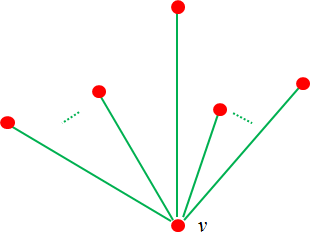
\includegraphics[width=0.6\linewidth]{figs/fork.png}
  \caption{\label{fig:fork}%
           A skeleton $S$ that is a fork originated from a node.}
\end{figure}

Now we claim that there is a clique cover in $G$ of size $K$ if and only if there is a skeleton partition of $S$ into $K$ support-free subgraphs(the angle between each pair of arcs is no larger than $2\theta$).
For if there is clique cover in $G$ of size $K$, then each clique in $G$ corresponds to a rooted subgraph of $S$ that satisfies the angle constraint. Conversely, if $S$ is partitioned into $K$ support-free subgraphs, then every pair of arcs in each subgraph satisfy the angle constraint, by the mapping relation, their corresponding nodes in $G$ form a clique. This completes the proof. \qed

This tells the difficulty of solving the problem of partitioning a 3D model into the least number of support free pieces. In the following, we shall show how to solve the problem with a practical yet efficient algorithm.

However, as the topology of the skeleton $S$ is a tree such that the degree of each node of the tree is no larger than a constant $d$, and the least number of support-free subgraphs is bounded by another constant $c$, then we show that the problem of partitioning $S$ into the least number of support-free subgraphs (satisfying the angle constraint) can be computed in polynomial time. In general, for a tree structure with arbitrary $c$ and $d$, we have them following theorem.

\emph{\textbf{Theorem 2}: Given three integer numbers $c$, $d$, Let $S$ be a tree structure such that the degree of each node is bounded by $d$, then whether $S$ has $c$ support-free subgraphs can be determined in $O(2^{cd}n^{2c})$ time, and a partition instance can be reported within the same time bound.}

\emph{Proof}: We shall prove the theorem by construction. In taking a subgraph from a tree structure $S$, we can duplicate a node $v$ and take a subset of arcs incident to it. Given a node with $d$ arcs incident to $v$, then the number of subsets of arcs incident to it is $C(d, 1) + C(d, 2) + ... + C(d, d-1) = O(2^d)$. 
In order to construct a partition of $S$ into $c$ subgraphs, we need to choose at most $c$ nodes from $S$ (it is possible that multiple subgraphs are derived from a common node). More precisely, we need to choose $i$ nodes for $1\leq i \leq c$, for each node there are $O(2^d)$ choices. Therefore, the number of all possible partitions is bounded by $O(\sum_{i=1}^{c}C(n, i)*2^{cd}= O(2^{cd}n^c)$.
For the resulting partition, we need to make sure that it is a valid partition, i.e., no two arcs are contained in more than one subgraph. This can be done in $O(n)$ time by counting the total number of arcs in the resulting partition: if it is equal to $(n-1)$, then the partition is valid; else otherwise. For each valid partition, we need to determine whether a subgraph is support-free. For this purpose, in each valid partition, for a subgraph of size $n_i$, it takes $O(n_i)$ time to check whether the subgraph is a support-free one given a node as the root. Therefore it takes $O(n_i^2)$ time for processing all nodes in the subgraph. In sum, it takes $O(\sum_{i=1}^{c}n_i^2) = O(n^2)$ time to check whether a partition is a support-free one. Therefore, for all $O(2^{cd}n^c)$ partitions, it requires $O(2^{cd}n^c*n^2) = O(2^{cd}n^{2c})$ time. This completes the proof \qed

As a result, if $c$ is a constant, then partitioning $S$ into $c$ support-free subgraphs can be done in polynomial time. Further, the least number of subgraphs can be determined by a standard binary operation on $c$. More precisely, if $c$ is sufficient to obtain a feasible support-free partition, then we can try $c/2$, and then $c/2^2$ if $c/2$ is also sufficient, and so on so forth, finally, a half interval is added back, and the number before and after this resulting number are used to locate the final value of the smallest number. The construction process in the proof of Theorem 1 directly suggests a polynomial time algorithm for computing the least number of support-free subgraphs when $S$ is a tree structure with constant $c$ and $d$.}}

We formulate the partition problem with the objectives of both the total number of cuts and the cutting length, under the constraint of printing angle of each branch with respect to the build platform, the angle between a cutting plane and the printing direction, the dimension of each printed model with respect to the printable volume of a given printer, and the base area of a printed model. Since the problem is NP-hard, we propose a randomized Monte Carlo method in compliance with a set of carefully designed selection strategy to seek a practical solution. Figure \ref{fig:ex1} shows an example of a deer model (shell), our partition result based on Laplacian skeleton of the model, the printing result and the assembly effect. The details of Monte Carlo method is given below.




\section{Algorithm}
%\textbf{Skeleton Partition.}
Let $M$ denote the mesh model, and let S denote the Laplacian skeleton obtained via the algorithm provided in \cite{AuTCCL08}. We propose an algorithm for partitioning $M$ into a minimum set of \emph{disjoint} components, each of which can be fabricated in a 3D printer without using any support structure. Decomposing $S$ into two pieces can be done by duplicating a node $v$; while partitioning $M$ at node $v$ requires the determination of the position and normal of a cutting plane. To guarantee an aesthetical look on the resulting surface with shortest seams, we need a constraint to minimize the peripheral length of the cut in terms of the position and normal of the cutting plane. Note that the orientation of the cutting plane affects the printing direction and thus the shape of the subgraph while on the contrary, the shape of the subgraph constrains the orientation of the cutting plane. Hence, this is an essential \emph{chicken-and-egg} problem. In addition, we also need to consider the printing volume limit, i.e., the volume of the printing model should be within the working volume of a given 3{D} printer.

To summarize, our objectives are the minimization of: (1) the number of partitioned components $N$ of the mesh model; (2) the total peripheral length of each cut $L_i$, i.e., $\Sigma L_i$. The constraints of the problem are as follows:


(i) Each arc of the partitioned subgraph $H_i$ subtends to an axis by an angle of no larger than $\theta$, where $\theta$ is a printer-dependent parameter obtained from experiments. This guarantees that the corresponding mesh component is support-free during the printing process;


(ii) As the directed arcs of $H_i$ are translated to a common origin, they form a fork (see Figure \ref{fig:cone}). Let $a$ and $b$ be the pair of farthest vectors in the fork, i.e., the angle between $a$ and $b$, denoted as $\alpha$, is the largest. Let the central ray of the minimum cone that encloses the fork be denoted as $r(H_i)$, then $r(H_i)$ is collinear with $a + b$. Then the feasible directions of printing $H_i$ without using any support is bounded by a solid cone centered at $r(H_i)$ with an apex angle of $2\theta - \alpha$ (Figure \ref{fig:cone}). Therefore, let $b(H_i)$ be the base cut of the mesh part that corresponds to the root of $H_i$ {(by base cut we mean the cutting boundary which adheres to the printing platform when the part is being printed, see Figure \ref{fig:ex1} (d))}, then $b(H_i)$ is orthogonal to some vector $\hat{e}$ in $cone(H_i)$. %This guarantees that the base can be placed on the 3D printing platform.

Thereafter, in order to guarantee support-free fabrication of any cut other than the base, the angle between any non-base cut and the base cut should be no larger than $\theta$ since the base cut determines the printing direction. More precisely, any other cut $c$ separating subgraph $H_i$ from another subgraph $H_j$ should satisfy the constraint that the angle between $c$ and $b(H_i)$ is no larger than $\theta$. Let $A(c, b(H_i))$ denote the angle, then $A(c, b(H_i)) \leq \theta$. Since a cut separates the mesh into two parts, possibly sacrificing the angle constraint of the mesh part corresponding to a subgraph adjacent to $H_i$, an additional cut respecting the angle constraint of the adjacent subgraph may be required. Detailed steps for addressing this issue is given in the section for Mesh Partition below.

\begin{figure}[t]
  \centering
  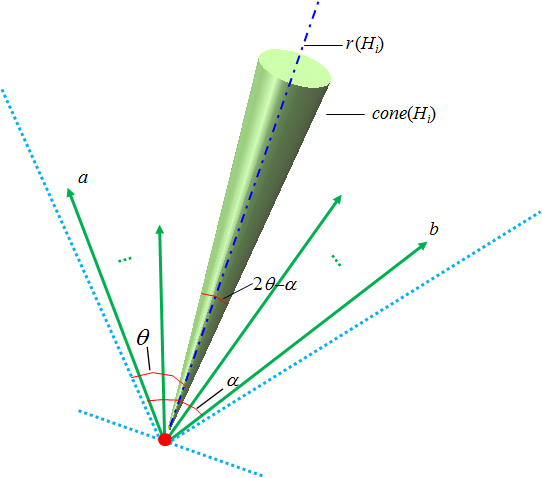
\includegraphics[width=0.7\linewidth]{figs/cone.png}
  \caption{\label{fig:cone}%
           Illustration of $r(H_i)$ and $cone(H_i)$.}
\end{figure}

%As a cut partitions a shell model, one facet is generated for the CAD model, but it two facets are generated physically, . Let the normal direction of the cut $c$ (pointing to the exterior of the partitioned part) be denoted as $n(c)$.

%Mathematically, a cut behaves as a single facet for the mesh; but it results in two facets on the appearance of the physical model. With the physical understanding, for each cut c, let $c_1$ and $c_2$ be the two facets on the physical model. Since $M$ is a shell mode, $c_1$ and $c_2$ are two annular-shaped plane facets. Let $n(c_1)$ be the normal direction of $c_1$ that points into the interior of the shell. $n(c_1)$ is defined similarly.


(iii) The base of a printing model should be large enough to gather sticky force from the building platform, such that the model is not deformed during the building process. Formally, let $area(b(H_i))$ denote the area of the base of the mesh component corresponding to $H_i$, which is approximately equal to the peripheral length of the base times the thickness of the shell. let $\tau$ be a user-defined threshold value, then we have $b(H_i) \geq \tau$. Here $\tau$ can be determined empirically; Finally,


(iv) Each cut partitions a single subgraph.

We have the following optimization system:
\begin{equation*}
\begin{aligned}
& \underset{x}{\text{minimize}} \quad N \quad \text{and} \quad \sum_{i=1}^N{L_i},
\quad \text{subject to:} \\
& A(e, r(H_i)) \leq \theta, \; i = 1, \ldots, m, \forall e \in H_i, & (1)\\
& b(H_i) \bot \hat{e}, \hat{e} \in cone(H_i), & (2)\\
& A(c, b(H_i)) \leq \theta, & (3)\\
& area(b(H_i)) \geq \tau, & (4)\\
& cut \cap S = cut \cap H_i, cut \in \{b(H_i), c\}  & (5)
\end{aligned}
\end{equation*}
where all $H_i$-s constitute a partition of the original graph. A direct exploration of all possible partitions over the graph $G$ could quickly leads to exponential complexity. The key here is to quickly find potential good partitions in a way that subsequent exploration of the graph is limited to those which leads to a less value of the optimization function. We employ a randomized Monte Carlo algorithm detailed below.

We separate the minimization of the two target terms sequentially, i.e., the number of mesh components and the total cutting length. In the following, we shall discuss how the skeleton and mesh are partitioned in details.

\textbf{Skeleton Partition.} To minimize the number of subgraphs,
we use a randomized exploration strategy, but give a higher probability to explore the graph broadly. In particular, assume that we are given a function $Trim\_BFS(v, G, \theta)$ which traverses $G$ from $v$ in a breath first search manner to progressively collect arcs which satisfy Constraint (1); and a function $MeshPartition(U , M)$ that decomposes $M$ based on the set of partitioned subgraphs $U$, and returns a partition of $M$, denoted as $M^{'}$, and the number of cuts $N$. Algorithm \ref{alg:Framwork} sketches the idea of the skeleton decomposition. The main idea is to randomly search for candidate subgraphs using Monte Carlo Method, which randomly chooses a node of $G$ to start traversing and randomly grows the subgraph while paying attention to the aforementioned constraints.

\begin{algorithm}
\caption{$Skeleton\_Mesh\_Decomposition(S, M)$}
\label{alg:Framwork}
\begin{algorithmic}[1]
\REQUIRE~
The Laplacian skeleton $S$ and mesh model $M$.
\ENSURE~
The decomposition of $M$ into the least pieces of components that are free of support.

%; a partition of $M$ based on $T$ that satisfies constraint (2-4)
\STATE $M_{opt} = \emptyset$; $min = \inf$; $count$ = 0; $max\_iter$ = a user defined large constant;
\WHILE {$count < max\_iter$}
\STATE  $U= \emptyset$;
\WHILE {$S\neq \emptyset$}
\FOR{$i=1$; $i<|| S ||$; $i++$ }
\STATE $H = Trim\_BFS(v_i, S, \theta)$;
\STATE $S = S / H$;
\STATE $U = U \cup H$;
\ENDFOR
\STATE $(M^{'}, N) = MeshPartition(U , M)$;
\IF {$N < min$}
\STATE  $min = N$;
\STATE  $M_{opt} = M^{'}$;
\ENDIF
\ENDWHILE
\STATE $count =count + 1$;
\ENDWHILE
\RETURN  $M_{opt}$;
\label{code:fram:select} \\
%\STATE call function $Mesh\_Decomposition(M, T)$;
\end{algorithmic}
\end{algorithm}




\begin{figure}[tbp]
  \centering
  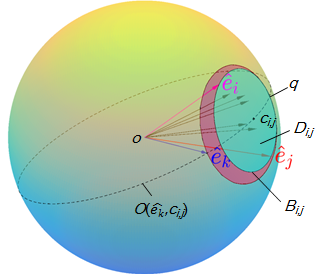
\includegraphics[width=\linewidth]{figs/take_arc.png}
  \caption{\label{fig:sphere}%
           Illustration of unit vectors, unit sphere, spherical disks, and the determination of taking a new edge in $Trim\_BFS$.}
\end{figure}

Next we shall show how $Trim\_BFS(v, G, \theta)$ works to find a locally maximal subgraph starting at $v$ that satisfies the angle constraint. Let $H$ be the current subgraph obtained so far. When an arc $e$ of $G$ is visited, we need to determine whether it should be included into $H$. If the start of each outgoing arc of $H$ is moved to a common origin, then the arcs form a fork of rays (Figure \ref{fig:sphere}). A naive method to judge whether $e$ should be included is to move the start of $e$ to the origin of the fork, and compute the angle between $e$ and each arc of the fork, $e$ is included if the maximum angle between $e$ and each arc of the fork does not exceed 2$\theta$. However, this would lead to $O(n^{2})$ time complexity of $Trim\_BFS(v, G, \theta)$, where $n$ is the size of $G$. To speed up this process, we keep the pair of vectors which form the largest angle and judge whether a new vector expands the angle of the fork. See Figure \ref{fig:sphere}, let $\hat{e_i}$  and $\hat{e_j}$ be the units of these two vectors obtained so far. For simplicity, we denoted by $F( \hat{e_i}, \hat{e_j} )$ the fork with the starts of all unit vectors converging at the origin of the coordinate frame, where $\hat{e_i}$  and  $\hat{e_j}$  are the pair of unit vectors that form the largest angle in the fork. Let $\hat{e_k}$  be the unit of a new vector to be processed next, if $\hat{e_k}$ penetrates through the blue circle, then no change need to be made to the fork; otherwise, let $D_{i,j}$ denote the spherical disk that passes through the endpoints of $\hat{e_i}$  and $\hat{e_j}$ whose central axis is collinear with $\hat{e_i}$  + $\hat{e_j}$, let $c_{i,j}$ be the center of $D_{i,j}$, let $B_{i,j}$ be the boundary circle of $D_{i,j}$. The circle passing through $\hat{e_k}$  and $c_{i,j}$, denoted as $O( \hat{e_k}, c_{i,j})$, intersects  $B_{i,j}$ at two points, let $q$ the point further away from the endpoint of $\hat{e_k}$, then $\overrightarrow{oq}$ and $\hat{e_k}$ are the two extreme vectors that to be used in the next iteration. To summarize, a new arc $e_k$ is taken by $Trim\_BFS$ if and only if one of the following two conditions is met:
(1) the angle between $\overrightarrow{oc_{i,j}}$ and $\hat{e_k}$, denoted as $A(\overrightarrow{oc_{i,j}}, \hat{e_k})$, satisfies  $A(\overrightarrow{oc_{i,j}}, \hat{e_k}) \leq A(\overrightarrow{oc_{i,j}}, \hat{e_i})$;
(2) $A(\overrightarrow{oq}, \hat{e_k})  \leq  2\theta$, where $q = O( \hat{e_k}, c_{i,j}) \cap B_{i,j}$.


\begin{algorithm}[t]
\caption{Algorithm: $Trim\_BFS(v, S,\theta)$}
\label{alg:trim}
\begin{algorithmic}[1]
\REQUIRE~
A node $v$ of Laplacian skeleton $S$, an angular value $\theta$.
\ENSURE~
 %A maximal subgraph $H$ rooted at $v$ and its corresponding mesh component that meet the constraints $(Eq.1-4)$.
 A subgraph $H$ rooted at $v$ that meets constraint (1).
\STATE starting from $v$, initialize F($\hat{e_i}$, $\hat{e_j}$); $H = \emptyset $;
\WHILE  {the current arc $e_k$ of $S$ picked by the BFS process is nonempty}
  \IF  {$A(\overrightarrow{oc_{i,j}},  \hat{e_k}) \leq A(\overrightarrow{oc_{i,j}},  \hat{e_i})$}
  \STATE  $H = H \cup \{e_k\}$;
  \ELSIF {$A(\overrightarrow{oq},  \hat{e_k}) \leq  2\theta$}
  \STATE $q = O( \hat{e_k}, c_{i,j}) \cap B_{i,j}$;
%  \IF  {$A(\overrightarrow{oq},  \hat{e_k}) \leq \pi- 2\theta$}
  \STATE  $\hat{e_i}=  \hat{e_k}$;
  \STATE $\hat{e_j} =  \overrightarrow{oq}$;
  \STATE  update $B_{i,j}$ and $c_{i,j}$;
  \STATE  $H = H \cup \{e_k\}$;
  \ENDIF
\ENDWHILE
%\STATE  call the cutting scheme for $M$;
%\STATE  $M= M/M_H$;
\label{code:fram:select} \\
%\RETURN  $H$ and $M_H$;
\RETURN  $H$;
\end{algorithmic}
\end{algorithm}

Algorithm \ref{alg:trim} demonstrates the growing process. Since the order of the chosen arcs influences the shape of the final BFS subgraph, in line $2$, the BFS process randomly chooses an arc incident to $v$ to proceed on. In order to guarantee a greater chance of converging to the optimal result in a short time, we refine Algorithm \ref{alg:trim} by inducing probabilities of choosing each arc of $S$. We denote this improved version of Algorithm \ref{alg:trim} as \textbf{$Trim\_BFS\_II$}. The main idea of $Trim\_BFS\_II$ is as follows.
We apply a training-and-learning procedure for the first $k$ (say $1000$) runs. Formally, let $n_v$ be the number of times an arc is chosen as the exit arc when node $v$ is visited. Given the data of the first $k$ runs, when a node $v$ is visited, the probability of choosing an arc $e$ as an outgoing arc in the subsequent runs is, $P(v, e) = n_v/k$.

%To further speed up the process of $Trim\_BFS$, we assign a mark that stores the minimum number of subgraphs obtained so far, such that the current branching can be terminated if its output number of subgraphs is larger than the mark.


Further, as $Trim\_BFS\_II$ is greedy, the growth is towards a local maximal subgraph that satisfies the angle constraints, the resulting partition of Algorithm \ref{alg:Framwork} might not be a global optimum. In order to ensure more possibilities to find a global optimum, we set a probability-based scheme to terminate the growing of a subgraph. The probability to terminate the growing is set to $r/n$, where $r$ is the size of the current subgraph and $n$ is the size of $G$. This gives high probability for $Trim\_BFS\_II$ to grow in larger sizes while rising the probability of exploring subgraphs of smaller sizes. We implemented it using rejection sampling.

%Since the traversing process assigns a specific direction to each arc that was originally undirected in $S$, it is not obvious whether the angle constraint is satisfied, To clarify this, we provide the following lemma.


%\begin{figure}[t]
%  \centering
%  \mbox{} \hfill
%  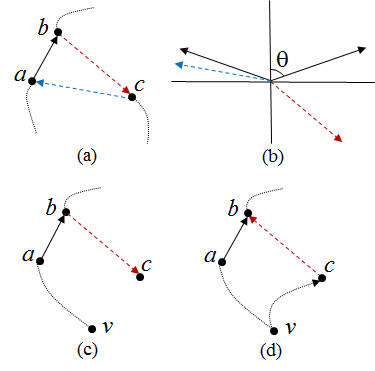
\includegraphics[width=0.4\textwidth]{figs/proof.png}
%  \caption{\label{fig:proof}%
%           Illustration of taking a directed arc into a maximal subgraph by $Trim\_BFS$.}
%\end{figure}



%\emph{Lemma 1}: $H = Trim\_BFS(v, G, \theta)$ is a maximal subgraph of $G$ that satisfies the angle constraint, i.e., each arc of $H$ subtends to an axis by an angle of no larger than $\theta$.


%\emph{Proof}: Suppose to the contrary that $H$ violates the angle constraint, there exists a directed arc that does not satisfy the angle constraint. For example, arc $\overrightarrow{ca}$ or arc $\overrightarrow{bc}$ in Figure \ref{fig:proof}. Such case is impossible as Line $3$ and Line $6$ of function $Trim\_BFS$ excludes any directed arc that violates the angle constraint of no larger than $\theta$ with respect to the (virtual) central axis.It remains to prove that $H$ is maximal, i.e., the largest graph rooted at $v$ that covers all the arcs that satisfies the angle constraint. Suppose that this is not true, there must exist an arc that was mistakenly discarded due to the direction in which the arc is traversed. Let $(b, c)$ be one of such arcs, as illustrated in Figure \ref{fig:proof}(a). When the arc is directed from $b$ to $c$, it is not included as it violates the angle constraint, but can be included if the arc directed from $c$ to $b$. We shall prove in a case-by-case basis. If $c$ is not reachable from $v$ via a directed path passing through $b$ (Figure \ref{fig:proof} (c)), then $c$ is only reachable from $b$, arc $bc$ should not be included and line 6 of Function $Trim\_BFS$ correctly handle this case. Otherwise, $c$ is reachable from $v$ via a directed path without passing through $b$ (Figure \ref{fig:proof} (d)). As $c$ is visited, by Line 2 of Function $Trim\_BFS$, each arc leaving $c$ is considered, and $\overrightarrow{cb}$ is correctly included into $H$. This completes the proof.



\begin{figure}[t]
  \centering
  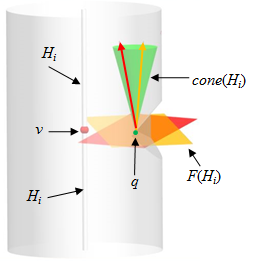
\includegraphics[width=0.3\textwidth]{figs/cone-fillet.png}
  \caption{\label{fig:fillets}%
           Illustration of a cone and its corresponding fillets, where two cutting planes in $F(H_i)$ and their associated vectors in $cone(H_i)$ are marked by distinct colors.}
\end{figure}


\textbf{Mesh Partition.}
{In the following section, we shall describe how MeshPartition(U , M) works as a cut is required around a skeleton node $v$. Codes are ommitted for brevity.}
The skeleton partition returns a set of nodes where the mesh partition should occur, in particular, the cutting plane should be in the vicinity of each node $v$ incident to at least two distinct subgraphs. We need to determine the exact positions and orientations of the cutting planes. For each node $v$ that is incident to at least two distinct subgraphs $H_i$ and $H_j$, we process it using the following cutting scheme.


Refer to Figure \ref{fig:fillets}, at the position of node $v$, we want to find a surface vertex $q \in M$ around $v$ through which the cutting plane should pass, while the cutting length is minimized. Let us denote the set of all planes which pass through a surface vertex $p$ and are orthogonal to vectors in $cone(H_i)$ (originated from $p$)  as $F(H_i)$, which we term as a \emph{fillet}. Then if the node $v$ is incident to two subgraphs $H_i$ and $H_j$, we have two plane sets $F(H_i)$ and $F(H_j)$ at point $p$, respectively. Depending on the position of $p$, we have the following two cases. \emph{Case (i)}: $F(H_i) \cap F(H_j) \neq \emptyset$. In this case, we shall randomly sample a set of cutting planes from $F(H_i) \cap F(H_j)$, and determine the one achieving the minimum cutting length; \emph{Case (ii):} $F(H_i) \cap F(H_j) = \emptyset$. In this case, two cuts are required in order to separate the mesh into support-free subparts. However, care must be taken as the angle between $c_1$ and $c_2$ should be constrained by $A(c_1, c_2) \leq \theta$. If this constraint is violated, one more cut in between $c_1$ and $c_2$ is required; while the base of each partitioned component should be no less than $\tau$. If any of the constraint is not satisfied, we shall translate the fillets along the printing direction in an opposite sense until the constraints are satisfied.

\begin{figure}[tbp]
  \centering
  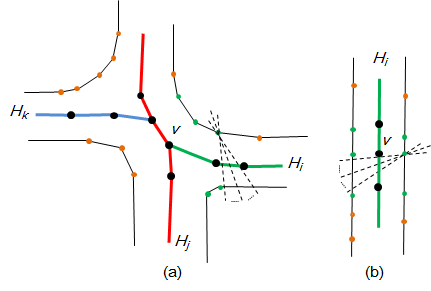
\includegraphics[width=0.5\textwidth]{figs/forward_tracing.png}
  \caption{\label{fig:forward_tracing}%
           2D illustration of $R(v)$ and the cuts, all vertices in $R(v)$ are shown in green, and the cuts associated with a vertex are shown in dashed lines:(a) the case of cuts around concave points; (b) the case of cuts on a cylindrical part.}
\end{figure}

In either case, a cut that nicely follows the geometry features is demanded in order to preserve aesthetic appearance in the final assembled object. We exploit shape concavity to look for a good cut as indicated by minima rule \cite{hoffman1984parts,hoffman1997salience}. However, the positions of the skeleton nodes may not locally reflect the geometric features such as concave areas on the mesh surface, therefore they are insufficient for a nice partition of the mesh. To compensate this, we exploit the concave vertices of the mesh that are incident to the skeleton nodes and take those that significantly concave into a candidate set of pivots for the cuts. More precisely, let $R(v)$ be the set of concave vertices on $M$ that are incident to $v$ during the Laplacian shrinking process \cite{AuTCCL08}, we truncate $R(v)$ such that the insignificant concave vertices are removed away. Here, given a vertex $v_i$ and any of its neighbor $v_j$, $v_i$ is concave if $(v_i - v_j)(n_j - n_i)$ is nonnegative, the significance of a concave vertex can be quantified as the magnitude of $(v_i - v_j)(n_j - n_i)$ \cite{au2012mesh}, denoted as $\tau_i$. We collect vertices whose $\tau_i$ is greater than a threshold $\delta$.

%See Figure \ref{fig:fillets}(c-d), for each vertex in $R(v)$, we shall process a pair of fillets as done for vertex $p$ above.


Next, we proceed to find a cutting plane around $v$. We first extend the region $R(v)$ by merging each $R(u)$ into it, where $u$ is an adjacent node of $v$ in $S$. Given all concave vertices in the new $R(v)$, each vertex defines a set of feasible cutting planes in accordance to its $fillet$. By feasible we require that a cutting plane does not cut through any other subgraph except for $H_i$. We then exhaustively go through all feasible cutting planes and find the one whose cutting length is minimum. In case of a cylindrical part that does not merit good concaveness, we reduce the threshold value $\delta$ by half and repeat the procedure until a feasible cutting plane with minimum length is found. Figure \ref{fig:forward_tracing} illustrates the process.


%Particularly, if $v$ is a leaf node that is merely neighbored to a single node $w$ in subgraph $H_i$, then the separation of the mesh component corresponding to $H_i$ may not be feasible if merely $R(v)$ is used, this is because the position of $v$ is chosen irrespective of the geometric features of the mesh. To separate the mesh component of $H_i$, we process arc $vw$ as follows: Given a user-defined threshold value $\delta$, if $| vw | \leq \delta$, then $R(v)$ is extended to contain the concave vertices of $M$ that are incident to $w$. On the other hand, if $| vw | > \delta$, then a partition of the arc $vw$ by an interval of $\delta$ is carried out. Subsequently, for each node along arc $vw$, the above scheme for processing node $v$ is exploited, see Figure \ref{fig:forward_tracing}. In this process, the tracing of the nodes along $vw$ stops as a cut does not intersect into any other subgraph other than $H_i$. The technique for detecting the intersection is as follows:

In order to determine whether a cutting plane cuts through any subgraph other than $H_i$, we take advantage of the correspondence between the mesh vertices and the skeleton nodes. Since each vertex of $M$ is mapped to a single node of $S$ \cite{AuTCCL08}, as a cut goes through the mesh surface, the endpoints of the edges of $M$ that are penetrated through give us the information of the potential subgraph that is cut through. Approximately, if a cut $c$ goes into an edge whose endpoints are incident to a subgraph $H_j$, then $c$ cuts through $H_j$.

%On the other hand, if $v$ is an internal node to at least two subgraphs, see Figure \ref{fig:cross}, then a partition of one subgraph around $v$ is inevitable. The partition scheme follows from the operations on the fillets.

Sometimes, it is possible for a mesh component which is not printable free of support even though its corresponding skeleton is detected to be printable free of support. This is because the skeleton piece that shares a junction node with some other subgraph may compromise its topology locally \cite{AuTCCL08}, and therefore cannot precisely describe the local topology feature of the partitioned component. In this case, we search along the skeleton and further partition it with an additional cut. Refer to Figure \ref{fig:arm} for an illustration. Empirically, we found this rarely happened.

\begin{figure}[tbp]
  \centering
  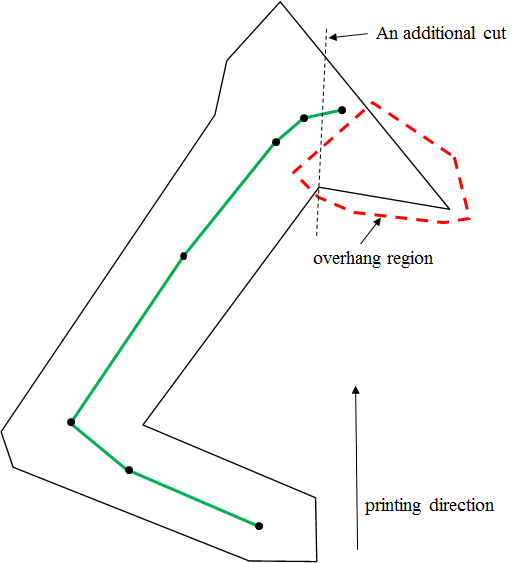
\includegraphics[width=0.3\textwidth]{figs/arm.png}
  \caption{\label{fig:arm}%
           Illustration of a mesh component with an overhange that requires support while its corresponding skeleton is support-free}
\end{figure}

%Finally, if the cut-subgraph constraint (Eq. (5)) is violated, a sequence of iterative cutting is required.










\section{Results}

Partition Examples: Without any partitioning operation, the inner and outer boundary of of a shell model needs to be filled by a huge amount of support materials in order to guarantee a fine surface quality. See Figure \ref{fig:dear-simulation} (a-b) for an illustration of the Sculpture model, both its inner and outer surface require significant amount of support in order not to be collapsed during the printing process; while our approach only keeps all cylindrical shells that are free of support (Figure \ref{fig:dear-simulation} (c-d)).

\begin{figure}[tbp]
  \centering
  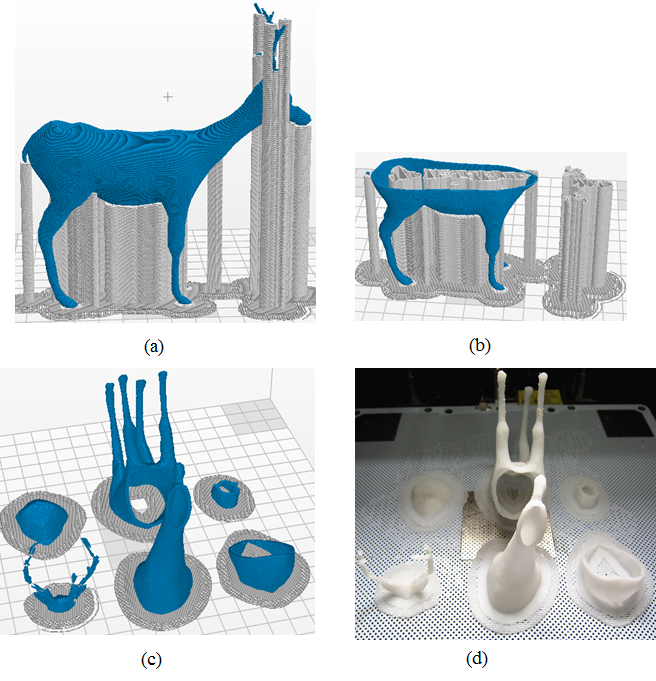
\includegraphics[width=\linewidth]{figs/dear-simulation.png}
  \caption{\label{fig:dear-simulation}%
           An illustration of the Sculpture model under the 3D printing software Z-suite as $\theta = 20^{\circ}$: (a) the full model; (b) an intermediate step of the simulation; (c) the simulation result of our partition for the Sculpture model; (d) the 3D printed result of our partition for the Sculpture model, no support is required.}
\end{figure}


\begin{figure}[tbp]
  \centering
  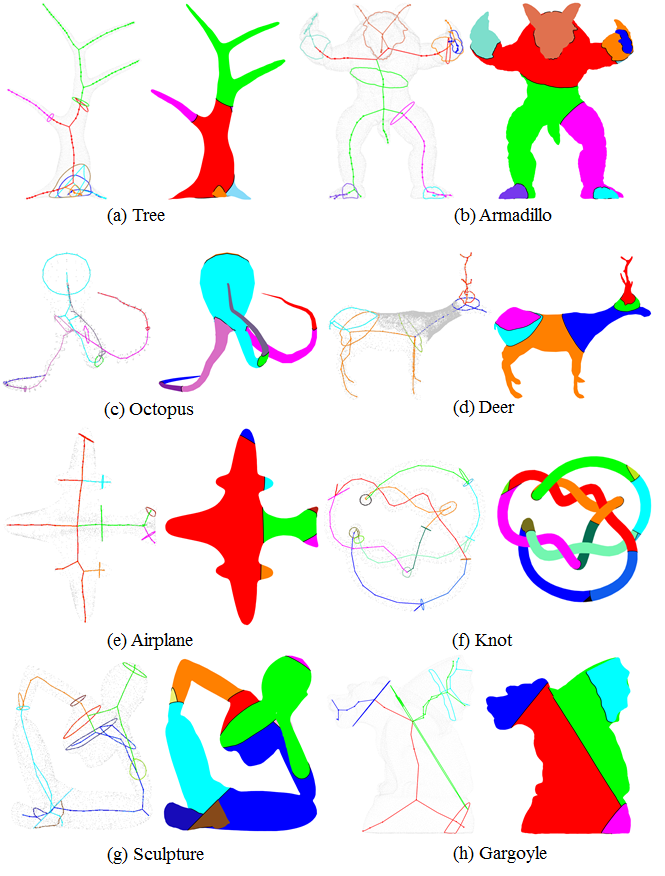
\includegraphics[width=0.45\textwidth]{figs/programming.png}
  \caption{\label{fig:programming}%
           Partition examples as $\theta = 70^{\circ}$. The printing direction of each part is orthogonal to its base (shown in the same color as the part)}
\end{figure}
We have run our algorithm on various natural or man-made models, and some of the results are presented in Figure \ref{fig:experiment}. We validated our approach by a set of printing experiments on Zortrax desktop printer, a kind of FDM machine that allows a printing layer thickness of 0.09mm , this is also the layer thickness we used in the printing experiments. The experiments are based on the choice of $\theta = 70^{\circ}$, i.e., all overhangs with an angle of no larger than $20^{\circ}$ with respect to the build platform are given support structures. Zortrax provides a built-in 3D printing software called \emph{Z-suite} can automatically counts the filament of the print material (in meters) and an estimate of the weight of the print material. Table \ref{tab:ertms:summary} summarizes the printing material and time costs by the original models and the partitioned models. Our approach significantly reduces both the printing material and time as the skeleton-based partition reduces both the supported materials inside and outside the models.


\begin{table*}[htb]

\begin{footnotesize}

\begin{center}

    \begin{tabular}{p{1cm} p{2cm} p{2cm} p{1.6cm} p{1.6cm} p{1.5cm} p{1.5cm} p{1.5cm} p{1.5cm}}

    \hline

     Models& Print material (original)& Print time (original)& Number of parts (skeleton partition)& Number of parts (mesh partition)& Print material (partition)& Print time (partition)& Material save (\%) &Time save(\%)\\ \hline
     Tree& 8.4m (20g)& 6h 32min &6 & 8 &5.19(12g) & 4h 2min & 38.2143 &38.2653\\ \hline
     Armadillo& 11.26m (27g)& 7h 30min &9 & 10  &4.65(11g) & 3h 30min & 58.7034 &53.3333\\ \hline
     Octopus& 12.82m (31g)& 10h 2min &5 & 9  &8.75(21g) &6h 51min & 31.7473 &31.7276\\ \hline
     Deer& 20.1m (48g)& 15h 8min &4 & 6  &8.89(21g) &5h 25min & 55.7711 &64.207\\ \hline
     Airplane& 11.56m (28g)& 6h 34min &5 & 7 &5.24(12g) &3h 10min & 54.6713 &51.7766\\ \hline
     Knots& 20.87m (50g)& 16h 50min &10 & 15 &12.38(29g) &11h 20min & 40.6804 &32.6733\\ \hline
     Sculpture& 23.68m (56g)& 18h 59min &4 & 10 &16.35(39g) &11h 23min & 30.9544 &40.0351\\ \hline
     Gargoyle& 8.76m (21g)& 6h 49min &4 & 5 &5.16(12g) &3h 48min & 41.0959 &44.2543\\ \hline

  \hline

    \end{tabular}

\end{center}

\end{footnotesize}

\caption{Statistics showing the print material, print time and partition number of the printed models.}\label{tab:ertms:summary}

\end{table*}


\begin{table*}[htb]

\begin{footnotesize}

\begin{center}

    \begin{tabular}{p{2.3cm} p{1.45cm} p{1.45cm} p{1.5cm} p{1.5cm} p{1.5cm} p{1.5cm} p{1.5cm}p{1.5cm}}

    \hline

     Models& Tree& Armadillo& Octopus& Deer& Airplane& Knots &Sculpture & Gargoyle\\ \hline
     number of vertices & 11443   & 34594   & 1343    & 8917  & 15485 & 2904    & 5979    &25002 \\ \hline
     running time(s)    &197.1732 & 311.559 & 97.1395 &90.618 &88.744 & 92.4798 &74.2186  &199.893 \\ \hline

  \hline

    \end{tabular}

\end{center}

\end{footnotesize}

\caption{The running time of processing the models.}\label{tab:ertms:time}

\end{table*}




\begin{figure}[tbp]
  \centering
  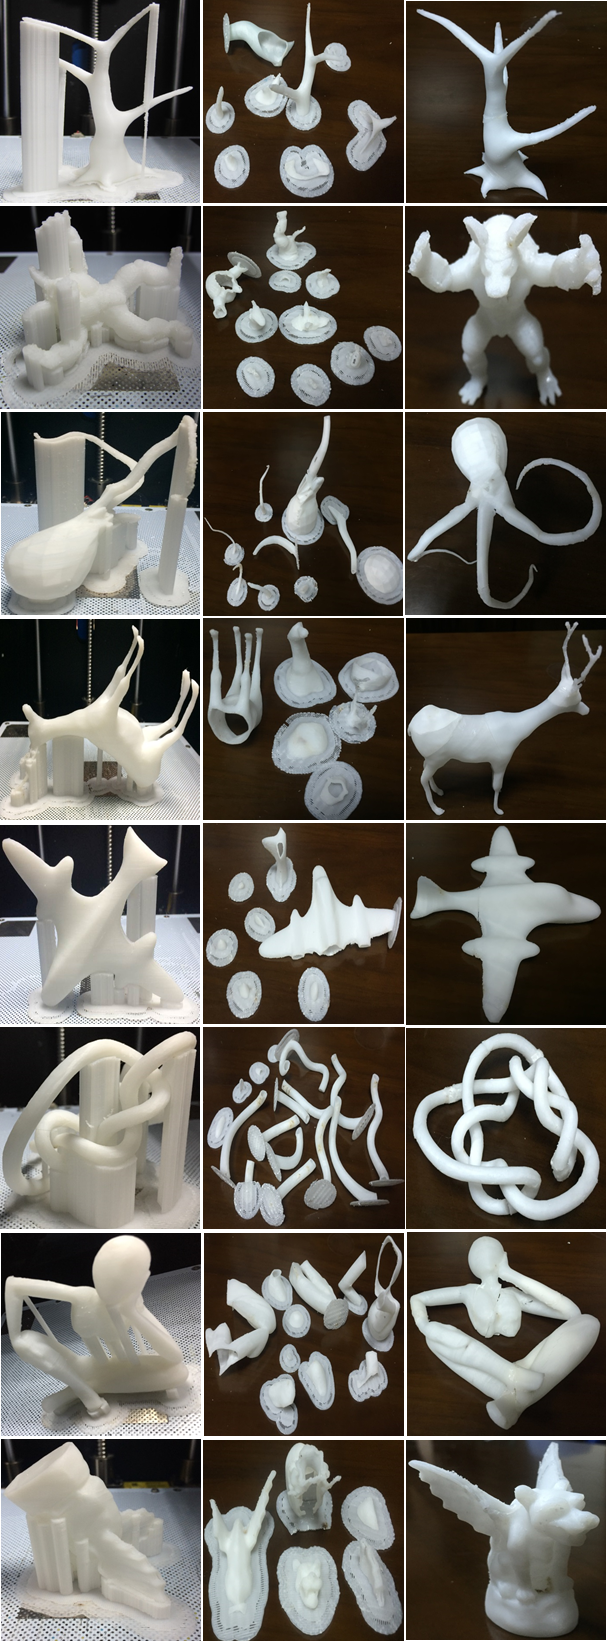
\includegraphics[width=0.48\textwidth]{figs/experiment.png}
  \caption{\label{fig:experiment}%
           A comparison between printing of original shell models and our partitioned models.}
\end{figure}

The algorithm was implemented with C++ on a PC with Intel i7-4790 and 8 GB RAM. The algorithm is run on each model for 8000 runs with the first 1000 runs taken as a training-and-learning process, the running time of processing the models are summarized in Table \ref{tab:ertms:time}. Figure \ref{fig:experiment} shows the comparison of the printing effects of the original models and our partitioned models. Due to the limit of the current technology, any FDM printer requires a small amount of supporting bed for holding the printed model on the printing platform, other printing techniques such as SLA, SLM and SLS may avoid the use of these supporting beds. Therefore, our approach guarantees support-free to the most extent for all exiting printing techniques.

\hl {[Evaluations: how close we are to the global optimum][Limitations: discussion about 1. the strength of our interior, -- future work. 2. cut through salient regions -- hard to balance. etc]} \youyi{We need some efforts in the paragraph below.}

Since the problem of partitioning the skeleton graph into the least number of support-free subgraphs is NP-hard, it is impossible to obtain an optimal result in polynomial time. However, from Table \ref{tab:ertms:summary}, we can conclude that the partition result for the skeletons are small enough. Particularly, which arcs to be taken into a subgraph and the taking sequence significantly affect the final partition result. From the programming result in Figure \ref{fig:programming}, it is very hard to identify how are away our partition result is from the optimal result (i.e., the least pieces of sub-skeletons), since an optimal partition result would require an enumeration of outrageously huge amount of combinations. However, we can evaluate our skeleton partition result by examining some simple skeleton examples with obvious optimal partition numbers.

Refer to Figure \ref{fig:cube}, the skeleton cannot be printed as a whole in a support-free manner due to the cross on the top facet. Our algorithm partitions the skeleton into two parts (shown in red and green respectively), and is therefore optimal. Note that the bars are hollow in the mesh model, therefore any support-free solid model based partition method (e.g., the one provided by \cite{Hu_siga14}) cannot be applied, and our skeleton-based partition method is preferable.

\begin{figure}[tbp]
  \centering
  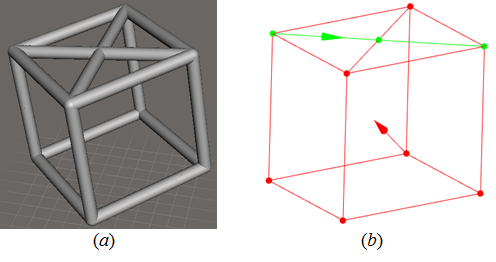
\includegraphics[width=0.4\textwidth]{figs/cube.png}
  \caption{\label{fig:cube}%
           An illustration of a shell model whose skeleton is partitioned into the least pieces by our algorithm.}
\end{figure}



%Further, our current approach of partitioning tries to find a node as a root of a subgraph, while in general it is possible that the subgraph is unrooted. For example, in Figure \ref{fig:unrooted}, under the angle constraint of $\theta = 70{\circ}$, the tree skeleton can be taken as a whole printable graph while our algorithm would take node $v$ as a root for the upper and lower parts of the tree respectively. Future research can be elaborated along this line. But how the general unrooted subgraphs are taken efficiently other than  searching in an exhaustive combinatorial manner to form a minimum set of subgraphs is unknown.

%\begin{figure}[tbp]
%  \centering
%  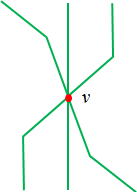
\includegraphics[width=0.2\textwidth]{figs/unrooted.png}
%  \caption{\label{fig:unrooted}%
%           An illustration of a tree skeleton that satisfies the angle constraint but is taken as two subgraphs by our algorithm.}
%\end{figure}

%However, we can evaluate the effectiveness of our approach by judging the topology of some simple models and evaluate how close our partition is from a potential optimal result. For example, from Figure \ref{fig:ex1}, under the requirement of $\theta = 70^{\circ}$, ignoring the tinny detailed geometric features we can observe that an optimal partition of the deer model requires at least $4$ cuts: the tail, the chunk including the legs, the neck, and the head and the horn. Our approach provides a partition of 4 cuts, which is almost near the optimal. Further, from the appearance of the gargoyle model (the last row of Figure \ref{fig:experiment}), we can see that an optimal cutting should have the following 4 parts: the head, two wings, and the remaining parts. Our partition results in 5 parts, which is very close to the potential optimal partition.

%Our approach is devoted to shell models, it can also be applied to cutting solid models without any problem. However, our approach suffers from a few limitations: for shell models, the thickness of the shells need to be large enough such that no serious deformation is caused during the assembling process. However, the problem of setting the minimum thickness of the model for various parts of the model is non-trivial, and our current work is restricted to a uniform setting of the shell thickness whose value is determined by an error-and-trial process. Further, the strength guarantee is not elaborated in this work, a possible solution is to use the algorithm in \cite{WangWYLTTDCL13} that distributes the least amount of materials for constructing a truss frame beneath the skin. Finally, our approach may allow a cut that passes through a salience region, which may hurt the appearance of the model. We found that it is difficult to make a balance between the saliency and the minimal cutting length as well as the minimal cutting numbers. A potential future research is to take care of salience region during graph partition. Finally, as a trade-off, a spatially curved cut might be a consideration to alleviate the salience problem.


\section{Conclusion}

In this paper, we present a skeleton-based approach for partitioning a model into part which are free of supporting structure when fabricated. We formulate the model partition problem into a constrained graph partition problem which is particularly tailored toward 3{D} fabrication. To tackle the NP-hardness of the problem, we exploit a randomized Monte Carlo method which adaptively searches for better partition possibilities while avoiding local minima. Compared with existing partition-based methods, the advantages of our partition method are as follows:

\begin{itemize}
 \item The models are support-free, especially for the 3D printing techniques including SLA, SLM and SLS. For FDM technique, it requires a bed of support that consumes very little volume of materials.
\item The seams on the assembled model are minimized in terms of cut number and cut length.
\end{itemize}

The support-free feature of our partition approach enables a significant amount of saving of the printing materials both inside and outside the model. Finally, our method is efficient and applicable to a large set of natural and man-made models.



%% The very first letter is a 2 line initial drop letter followed
%% by the rest of the first word in caps (small caps for compsoc).
%%
%% form to use if the first word consists of a single letter:
%% \IEEEPARstart{A}{demo} file is ....
%%
%% form to use if you need the single drop letter followed by
%% normal text (unknown if ever used by IEEE):
%% \IEEEPARstart{A}{}demo file is ....
%%
%% Some journals put the first two words in caps:
%% \IEEEPARstart{T}{his demo} file is ....
%%
%% Here we have the typical use of a "T" for an initial drop letter
%% and "HIS" in caps to complete the first word.
%\IEEEPARstart{T}{his} demo file is intended to serve as a ``starter file''
%for IEEE Computer Society journal papers produced under \LaTeX\ using
%IEEEtran.cls version 1.8a and later.
%% You must have at least 2 lines in the paragraph with the drop letter
%% (should never be an issue)
%I wish you the best of success.
%
%\hfill mds
%
%\hfill September 17, 2014



% An example of a floating figure using the graphicx package.
% Note that \label must occur AFTER (or within) \caption.
% For figures, \caption should occur after the \includegraphics.
% Note that IEEEtran v1.7 and later has special internal code that
% is designed to preserve the operation of \label within \caption
% even when the captionsoff option is in effect. However, because
% of issues like this, it may be the safest practice to put all your
% \label just after \caption rather than within \caption{}.
%
% Reminder: the "draftcls" or "draftclsnofoot", not "draft", class
% option should be used if it is desired that the figures are to be
% displayed while in draft mode.
%
%\begin{figure}[!t]
%\centering
%\includegraphics[width=2.5in]{myfigure}
% where an .eps filename suffix will be assumed under latex,
% and a .pdf suffix will be assumed for pdflatex; or what has been declared
% via \DeclareGraphicsExtensions.
%\caption{Simulation results for the network.}
%\label{fig_sim}
%\end{figure}

% Note that IEEE typically puts floats only at the top, even when this
% results in a large percentage of a column being occupied by floats.
% However, the Computer Society has been known to put floats at the bottom.


% An example of a double column floating figure using two subfigures.
% (The subfig.sty package must be loaded for this to work.)
% The subfigure \label commands are set within each subfloat command,
% and the \label for the overall figure must come after \caption.
% \hfil is used as a separator to get equal spacing.
% Watch out that the combined width of all the subfigures on a
% line do not exceed the text width or a line break will occur.
%
%\begin{figure*}[!t]
%\centering
%\subfloat[Case I]{\includegraphics[width=2.5in]{box}%
%\label{fig_first_case}}
%\hfil
%\subfloat[Case II]{\includegraphics[width=2.5in]{box}%
%\label{fig_second_case}}
%\caption{Simulation results for the network.}
%\label{fig_sim}
%\end{figure*}
%
% Note that often IEEE papers with subfigures do not employ subfigure
% captions (using the optional argument to \subfloat[]), but instead will
% reference/describe all of them (a), (b), etc., within the main caption.
% Be aware that for subfig.sty to generate the (a), (b), etc., subfigure
% labels, the optional argument to \subfloat must be present. If a
% subcaption is not desired, just leave its contents blank,
% e.g., \subfloat[].


% An example of a floating table. Note that, for IEEE style tables, the
% \caption command should come BEFORE the table and, given that table
% captions serve much like titles, are usually capitalized except for words
% such as a, an, and, as, at, but, by, for, in, nor, of, on, or, the, to
% and up, which are usually not capitalized unless they are the first or
% last word of the caption. Table text will default to \footnotesize as
% IEEE normally uses this smaller font for tables.
% The \label must come after \caption as always.
%
%\begin{table}[!t]
%% increase table row spacing, adjust to taste
%\renewcommand{\arraystretch}{1.3}
% if using array.sty, it might be a good idea to tweak the value of
% \extrarowheight as needed to properly center the text within the cells
%\caption{An Example of a Table}
%\label{table_example}
%\centering
%% Some packages, such as MDW tools, offer better commands for making tables
%% than the plain LaTeX2e tabular which is used here.
%\begin{tabular}{|c||c|}
%\hline
%One & Two\\
%\hline
%Three & Four\\
%\hline
%\end{tabular}
%\end{table}


% Note that the IEEE does not put floats in the very first column
% - or typically anywhere on the first page for that matter. Also,
% in-text middle ("here") positioning is typically not used, but it
% is allowed and encouraged for Computer Society conferences (but
% not Computer Society journals). Most IEEE journals/conferences use
% top floats exclusively.
% Note that, LaTeX2e, unlike IEEE journals/conferences, places
% footnotes above bottom floats. This can be corrected via the
% \fnbelowfloat command of the stfloats package.




% if have a single appendix:
%\appendix[Proof of the Zonklar Equations]
% or
%\appendix  % for no appendix heading
% do not use \section anymore after \appendix, only \section*
% is possibly needed

% use appendices with more than one appendix
% then use \section to start each appendix
% you must declare a \section before using any
% \subsection or using \label (\appendices by itself
% starts a section numbered zero.)
%


%\appendices
%\section{Proof of the First Zonklar Equation}
%Appendix one text goes here.

%% you can choose not to have a title for an appendix
%% if you want by leaving the argument blank
%\section{}
%Appendix two text goes here.


% use section* for acknowledgment
\ifCLASSOPTIONcompsoc
  % The Computer Society usually uses the plural form
  \section*{Acknowledgments}
\else
  % regular IEEE prefers the singular form
  \section*{Acknowledgment}
\fi


The authors would like to thank...

This work was supported in part by Shanghai Sailing Program No.16YF1405500, Shanghai Jiao Tong University Grant No. AF0200163, and State Key Laboratory of Mechanical Systems and Vibration Grant no. MSVZD201505.


% Can use something like this to put references on a page
% by themselves when using endfloat and the captionsoff option.
\ifCLASSOPTIONcaptionsoff
  \newpage
\fi


\bibliographystyle{IEEEtran}
\bibliography{skeleton_printing}


%% trigger a \newpage just before the given reference
%% number - used to balance the columns on the last page
%% adjust value as needed - may need to be readjusted if
%% the document is modified later
%%\IEEEtriggeratref{8}
%% The "triggered" command can be changed if desired:
%%\IEEEtriggercmd{\enlargethispage{-5in}}
%
%% references section
%
%% can use a bibliography generated by BibTeX as a .bbl file
%% BibTeX documentation can be easily obtained at:
%% http://www.ctan.org/tex-archive/biblio/bibtex/contrib/doc/
%% The IEEEtran BibTeX style support page is at:
%% http://www.michaelshell.org/tex/ieeetran/bibtex/
%%\bibliographystyle{IEEEtran}
%% argument is your BibTeX string definitions and bibliography database(s)
%%\bibliography{IEEEabrv,../bib/paper}
%%
%% <OR> manually copy in the resultant .bbl file
%% set second argument of \begin to the number of references
%% (used to reserve space for the reference number labels box)
%\begin{thebibliography}{1}
%
%\bibitem{IEEEhowto:kopka}
%H.~Kopka and P.~W. Daly, \emph{A Guide to \LaTeX}, 3rd~ed.\hskip 1em plus
%  0.5em minus 0.4em\relax Harlow, England: Addison-Wesley, 1999.
%
%\end{thebibliography}
%
%% biography section
%%
%% If you have an EPS/PDF photo (graphicx package needed) extra braces are
%% needed around the contents of the optional argument to biography to prevent
%% the LaTeX parser from getting confused when it sees the complicated
%% \includegraphics command within an optional argument. (You could create
%% your own custom macro containing the \includegraphics command to make things
%% simpler here.)
%%\begin{IEEEbiography}[{\includegraphics[width=1in,height=1.25in,clip,keepaspectratio]{mshell}}]{Michael Shell}
%% or if you just want to reserve a space for a photo:
%
%\begin{IEEEbiography}{Michael Shell}
%Biography text here.
%\end{IEEEbiography}
%
%% if you will not have a photo at all:
%\begin{IEEEbiographynophoto}{John Doe}
%Biography text here.
%\end{IEEEbiographynophoto}
%
%% insert where needed to balance the two columns on the last page with
%% biographies
%%\newpage
%
%\begin{IEEEbiographynophoto}{Jane Doe}
%Biography text here.
%\end{IEEEbiographynophoto}
%
%% You can push biographies down or up by placing
%% a \vfill before or after them. The appropriate
%% use of \vfill depends on what kind of text is
%% on the last page and whether or not the columns
%% are being equalized.
%
%%\vfill
%
%% Can be used to pull up biographies so that the bottom of the last one
%% is flush with the other column.
%%\enlargethispage{-5in}


%\begin{IEEEbiography}[{\includegraphics[width=1in,height=1.25in,clip,keepaspectratio]{figure/bio/lmm.jpg}}]{Minmin Lin} received the bachelor's degree in digital media technology from Zhejiang Sci-Tech University, Hangzhou, China, in 2012. Currently, she is working toward the PhD degree at Graphics and Parallel Systems Lab, Zhejiang University. Her research interests include modeling, object recognition and structure analysis.
%\end{IEEEbiography}

%\begin{IEEEbiography}[{\includegraphics[width=1in,height=1.25in,clip,keepaspectratio]{figure/bio/tianjia.jpg}}]{Tianjia Shao} is currently an Assistant Researcher in the State Key Lab of CAD\&CG, Zhejiang University. He received his PhD in Computer Science from Institute for Advanced Study, and his B.S. from the Department of Automation, both in Tsinghua University. His research interests include RGBD image processing, indoor scene modeling, structure analysis and 3D model retrieval.
%\end{IEEEbiography}

\begin{IEEEbiography}[{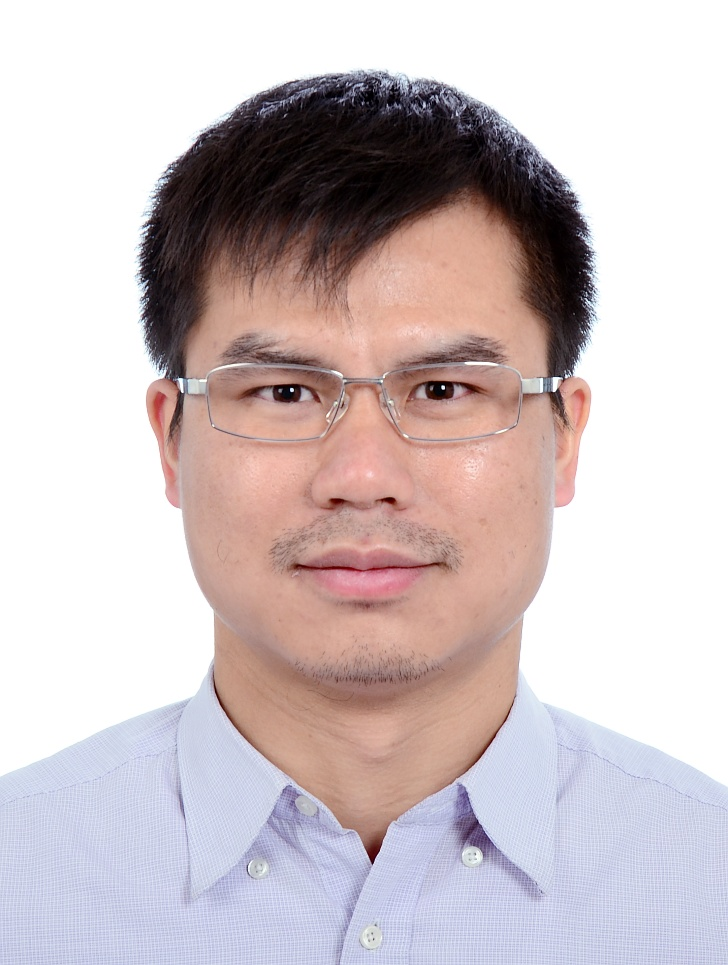
\includegraphics[width=1in,height=1.25in,clip,keepaspectratio]{figs/bio/wei.jpg}}]{Xiangzhi Wei} is an Assistant Professor with the Institute of Intelligent
Manufacturing and Information Engineering, School of Mechanical Engineering, Shanghai Jiao Tong University. He received his PhD and MPhil degree in Industrial Engineering and Logistics Management from the Hong Kong University of Science and Technology; and BE degree in Mechanical Engineering from Beijing Jiao Tong University. His current research interests include Additive Manufacturing (3D printing), computational geometry, algorithm design and analysis.
\end{IEEEbiography}
\begin{IEEEbiography}[{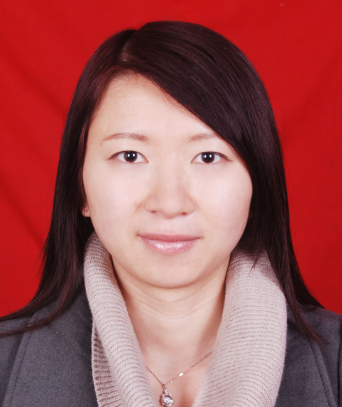
\includegraphics[width=1in,height=1.25in,clip,keepaspectratio]{figs/bio/qiu.png}}]{Siqi Qiu} is currently an Assistant Professor with the Institute of Intelligent
Manufacturing and Information Engineering, School of Mechanical Engineering, Shanghai Jiao Tong University. She received her PhD degree from the Department of Computer Engineering, Compiegne University of Technology, her MSc degree from Department of Electronic Engineering, University of Paris-Sud, and her BSc degree from School of Optical Science and Engineering, Huazhong University of Science and Technology. Her research interests include Monte Carlo methods, System of Systems, and reliability analysis under uncertainty.
\end{IEEEbiography}
\begin{IEEEbiography}[{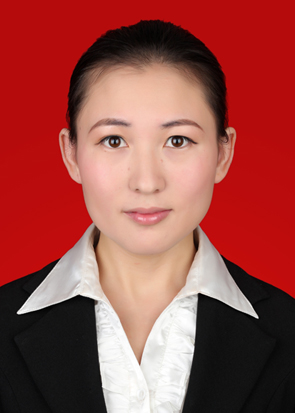
\includegraphics[width=1in,height=1.25in,clip,keepaspectratio]{figs/bio/zhu.jpg}}]{Lin Zhu} is a  PhD Candidate with the Institute of Intelligent Manufacturing and Information Engineering, School of Mechanical Engineering, Shanghai Jiao Tong University. She received her ME degree in Mechanical Engineering from the Xi��an Jiao Tong University; and BE degree in Packaging Engineering from Xi'an University of Technology. Her current research interests include Additive Manufacturing, Design of Experiments and Analysis.
\end{IEEEbiography}
\begin{IEEEbiography}[{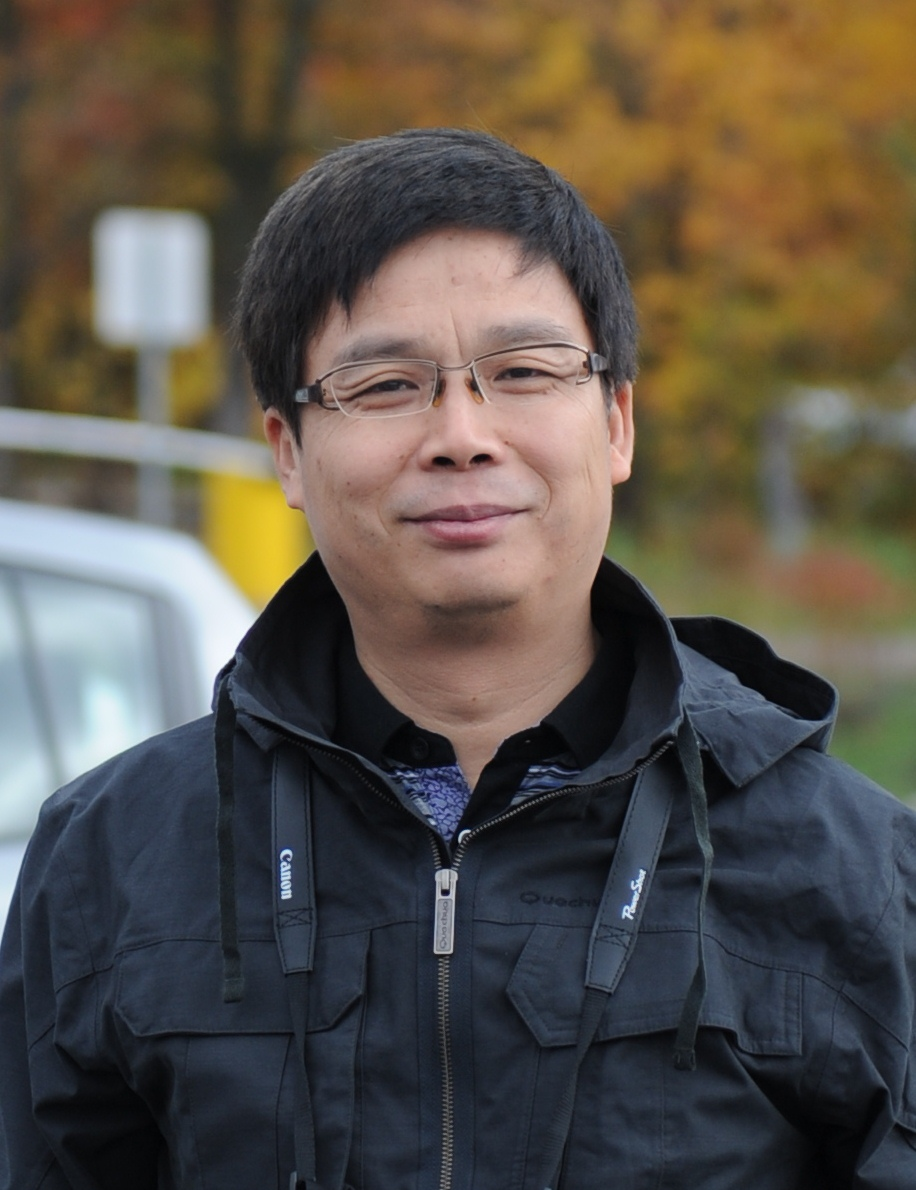
\includegraphics[width=1in,height=1.25in,clip,keepaspectratio]{figs/bio/xi.jpg}}]{Juntong Xi} received his PhD degree in Mechanical Engineering from Xi'an Jiaotong University. He is a full Professor with the Institute of Intelligent Manufacturing and Information Engineering, School of Mechanical Engineering, Shanghai Jiaotong University, Shanghai, China. His current research interests include digital manufacturing, measurement technology and instruments, and dental CAD.
\end{IEEEbiography}
\begin{IEEEbiography}[{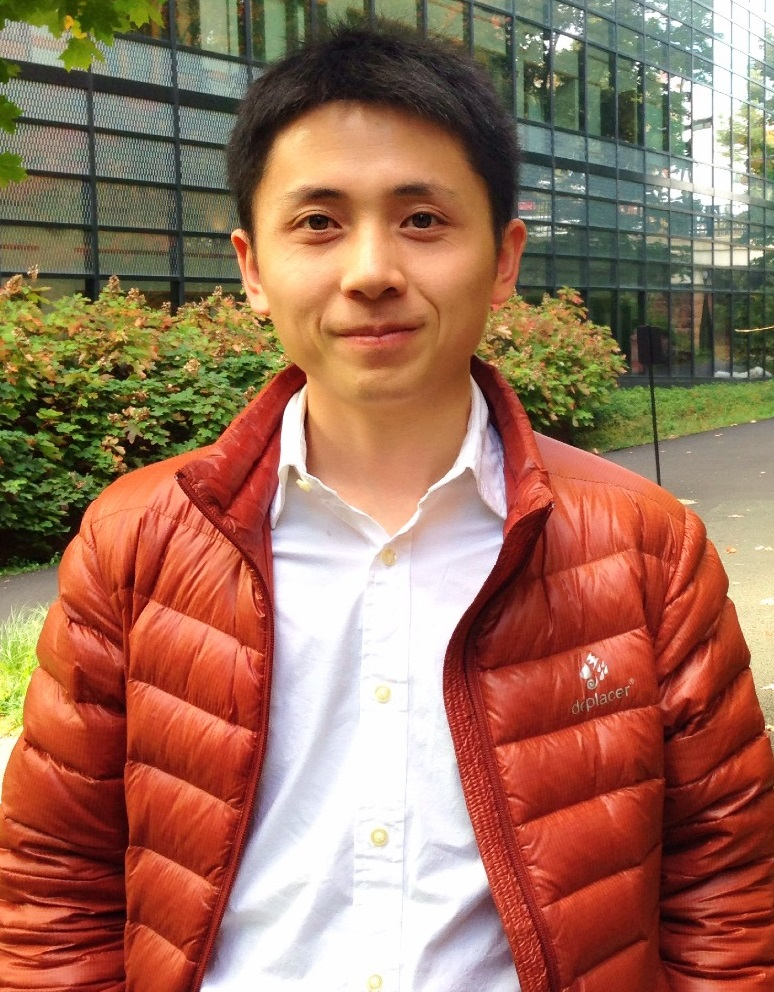
\includegraphics[width=1in,height=1.25in,clip,keepaspectratio]{figs/bio/yyz.jpg}}]{Youyi Zheng} is currently an Assistant Professor at the School of Information Science and Technology, ShanghaiTech University. He obtained his PhD from the Department of Computer Science and Engineering at Hong Kong University of Science \& Technology, and his M.Sc. and B.Sc. degrees from the Department of Mathematics, Zhejiang University. His research interests include geometric modeling, imaging, and human-computer interaction.
\end{IEEEbiography}


%\begin{IEEEbiography}[{\includegraphics[width=1in,height=1.25in,clip,keepaspectratio]{figure/bio/niloy.jpg}}]{Niloy J. Mitra} is a Professor of Computer Science at University College London (UCL). His research focuses on algorithmic issues in shape analysis and geometry processing. He received the ACM SIGGRAPH Significant New Researcher award in 2013 and the BCS Roger Needham award in 2015.
%\end{IEEEbiography}

%\begin{IEEEbiography}[{\includegraphics[width=1in,height=1.25in,clip,keepaspectratio]{figure/bio/kun.pdf}}]{Kun Zhou} is a Cheung Kong Professor in the Computer Science Department of Zhejiang University, and the Director of the State Key Lab of CAD\&CG. Prior to joining Zhejiang University in 2008, Dr. Zhou was a Leader Researcher of the Internet Graphics Group at Microsoft Research Asia. He received his B.S. degree and Ph.D. degree in computer science from Zhejiang University in 1997 and 2002, respectively. His research interests are in visual computing, parallel computing, human computer interaction, and virtual reality. He currently serves on the editorial/advisory boards of ACM Transactions on Graphics and IEEE Spectrum. He is a Fellow of IEEE.
%\end{IEEEbiography}

% that's all folks
\end{document}


